\documentclass[preprint,12pt]{elsarticle}
\usepackage{amsmath,amssymb,amsthm,mathtools}
\usepackage{booktabs,array,multirow}
\usepackage{graphicx}
\graphicspath{{../figures/}}
\usepackage{tikz}
\usepackage{hyperref}
\hypersetup{hidelinks}
\usepackage{microtype}
\usepackage[letterpaper,left=0.80in,right=0.80in,top=0.72in,bottom=0.78in]{geometry}
\usepackage{xcolor}
\usepackage{enumitem}
\usepackage{siunitx}
\usepackage{placeins}
\journal{Journal of Scientific Computing}

\newtheorem{theorem}{Theorem}[section]
\newtheorem{proposition}[theorem]{Proposition}
\newtheorem{lemma}[theorem]{Lemma}
\newtheorem{corollary}[theorem]{Corollary}
\newtheorem{remark}[theorem]{Remark}
\newtheorem{assumption}[theorem]{Assumption}
\newcommand{\PP}{\mathbb P}
\newcommand{\Th}{\mathcal T_h}
\newcommand{\D}{\mathcal D}
\newcommand{\Rn}{\mathbb R}
\newcommand{\grad}{\nabla}
\newcommand{\norm}[1]{\left\lVert #1\right\rVert}
\newcommand{\abs}[1]{\left\lvert #1\right\rvert}

\begin{document}
\begin{frontmatter}

\title{A High-Order $C^0$ Bernstein Quasi-Trefftz Method for Stationary Hamilton--Jacobi Equations}

\author[1]{Shelvean Kapita\corref{cor1}}
\ead{kapita@tamu.edu}
\cortext[cor1]{Corresponding author}
\address[1]{Department of Mathematics, Texas A\&M University, College Station, Texas, USA}

\begin{abstract}
We develop a high-order Bernstein--B\'ezier discretization for stationary Hamilton--Jacobi equations in which global continuity is imposed before the nonlinear equation is enforced.  The trial functions belong to an ordinary globally assembled continuous polynomial spline space on a triangulation, while element residuals are tested against polynomials one degree lower than the trial degree.  The degree shift is intrinsic to the first-order Hamiltonian structure: derivatives of degree-$p$ Bernstein polynomials are represented exactly in the degree-$(p-1)$ Bernstein basis, and linearization about a smooth branch produces transport in the characteristic direction given by the momentum derivative of the Hamiltonian.  Under a local transversality condition, a characteristic deep block is invertible and leaves a trace-sized tangent nullity of $p+1$ in two dimensions.  We prove local high-order approximation for smooth branches under general twice differentiable Hamiltonians, quantify perturbations caused by Hamiltonian approximation, and give a stability estimate for the implicit conforming qT condensation in terms of the smallest singular value of its selected characteristic block.  A direct parent-space comparison on a rotating-anisotropy Hamiltonian uses a rank-revealing implicit condensation of the assembled $C^0$ coordinates: an independent degree-$(p-1)$ moment block is satisfied to roundoff while the remaining coefficients are reconstructed as dependent conforming coordinates.  The resulting embedded $C^0$ quasi-Trefftz (qT) manifold preserves the high-order approximation trend of the full parent space.  Two non-eikonal manufactured Hamiltonians verify the general construction.  The eikonal equation is then used as the principal numerical study, including heterogeneous propagation, analytic point sources, a two-source first-arrival interface, the Marmousi velocity model, a factored focal caustic, and phase reconstruction at carrier frequencies up to 20000.  On Marmousi we use a causal coarse-grid solve only to select the viscosity branch and then apply Bernstein correction on successively refined triangulations; the experiment exposes both the gain from high-order branch correction and the error floor created by nonsmooth first arrivals.  The qT implementation uses batched element kernels, a fixed sparse global Jacobian pattern, one-time rank-revealing row selection, and sparse Newton condensation of the dependent conforming coefficients.  The earlier full-residual branch-correction prototype is retained for selected causal stress tests, where column-scaled Gauss--Newton/LSMR and inexact correction are useful for branch preservation.
\end{abstract}

\begin{keyword}
stationary Hamilton--Jacobi equation \sep eikonal equation \sep Bernstein--B\'ezier polynomials \sep quasi-Trefftz method \sep high-order approximation \sep caustics \sep geometric optics
\end{keyword}
\end{frontmatter}

\section{Introduction}
We consider stationary first-order Hamilton--Jacobi equations of the form
\begin{equation}\label{eq:HJ}
  H(x,\grad u(x))=0,\qquad x\in\Omega\subset\Rn^2,
\end{equation}
with boundary or inflow data selecting the branch of interest.  The isotropic eikonal equation
\begin{equation}\label{eq:eikonal}
  \abs{\grad u(x)}=n(x),\qquad n(x)>0,
\end{equation}
is the principal model in this paper.  It is obtained from the smooth Hamiltonian
\begin{equation}\label{eq:Heik}
 H_{\rm eik}(x,p)=\frac12\bigl(|p|^2-n(x)^2\bigr).
\end{equation}
Throughout, $x=(x_1,x_2)^T$ denotes position and $p=(p_1,p_2)^T$ the momentum variable.  We write $H_p$ for the gradient of $H$ with respect to $p$ and $H_{pp}$ for its momentum Hessian.  For a sufficiently smooth function $v$, define the Hamiltonian residual operator $\mathcal H(v)(x):=H(x,\grad v(x))$; thus $D\mathcal H(u)[w]$ denotes its Fr\'echet derivative at $u$ in the direction $w$.
Stationary Hamilton--Jacobi equations arise in optimal control, front propagation, geometrical optics, seismology, path planning, and differential games.  Their solutions may lose differentiability even for smooth data, so global first-arrival solutions are naturally interpreted in the viscosity sense; see Crandall--Ishii--Lions~\cite{CrandallIshiiLions1992} and the convergence framework of Barles--Souganidis~\cite{BarlesSouganidis1991}.  For the eikonal equation, the relation between phase, rays, geometrical optics, and high-frequency asymptotics is reviewed by Engquist--Runborg~\cite{EngquistRunborg2003} and Runborg~\cite{Runborg2007}.

The numerical Hamilton--Jacobi literature contains several complementary strategies.  High-order ENO methods were developed by Osher--Shu~\cite{OsherShu1991}; triangular-mesh formulations include the monotone and positive-coefficient constructions of Barth--Sethian~\cite{BarthSethian1998}, Abgrall's unstructured discretizations~\cite{Abgrall1996,Abgrall2009}, and central WENO schemes~\cite{LevyNayakShuZhang2006}.  Conforming finite-element ideas include the local variational method of Bornemann--Rasch~\cite{BornemannRasch2006}.  Discontinuous Galerkin formulations include Hu--Shu~\cite{HuShu1999}, the analysis of Lepsky--Hu--Shu in \emph{Applied Numerical Mathematics}~\cite{LepskyHuShu2000}, and the direct DG formulation of Cheng--Shu~\cite{ChengShu2007}.  Filtered schemes provide another route to combining viscosity-solution convergence with higher formal accuracy in smooth regions~\cite{ObermanSalvador2015}.

For static problems, causality can be exploited much more aggressively.  Tsitsiklis developed Dijkstra-type algorithms for discretized Hamilton--Jacobi equations~\cite{Tsitsiklis1995}; fast marching was introduced by Sethian~\cite{Sethian1996,Sethian1999}; ordered upwind methods extend causal ordering to broader anisotropic Hamiltonians~\cite{SethianVladimirsky2003}; and fast sweeping uses alternating characteristic-aligned Gauss--Seidel orderings~\cite{Zhao2005,KaoOsherTsai2005,ZhangZhaoQian2006,QianZhangZhao2007}.  Hybrid two-scale strategies combine marching and sweeping behavior~\cite{ChaconVladimirsky2012}.  These methods remain the natural choice when the primary objective is a robust viscosity solution on a very large grid.  The Bernstein method studied here is not intended to replace that role: it is a high-order solver for a selected smooth branch, and the two technologies are complementary rather than competing.

The present paper addresses a different regime.  We seek a high-order \emph{branch solver} for regions in which a classical Hamilton--Jacobi branch is smooth.  The starting point is an ordinary globally continuous Bernstein polynomial space.  The Hamiltonian is then used to remove locally resolvable residual directions through degree-$(p-1)$ moments.  This resembles quasi-Trefftz constructions in the sense that the PDE is built into a reduced polynomial representation, but the first-order nonlinear setting leads to a local manifold rather than a linear Trefftz space.  Polynomial quasi-Trefftz constructions for linear variable-coefficient PDEs provide useful precedent for the residual-adapted viewpoint~\cite{ImbertGerardDespres2014,ImbertGerardMoiolaStocker2023,ImbertGerardSylvand2025,ImbertGerardEtAl2025}.  A conformity-first Bernstein quasi-Trefftz construction for heterogeneous Helmholtz problems, in which exact $C^1$ Bernstein--B\'ezier smoothness is imposed before the PDE reduction, was developed in~\cite{KapitaC1BernsteinQT2026}; the present first-order $C^0$ construction is distinct, but it follows the same principle of carrying out equation-adapted reduction inside an already conforming Bernstein space.  Below we abbreviate quasi-Trefftz by qT when referring to the reduced/tangent construction.  Bernstein coordinates are particularly convenient because differentiation, edge restriction, and continuity are sparse coefficient operations; see Farin~\cite{Farin2002} and Lai--Schumaker~\cite{LaiSchumaker2007}.

The central observation is that the degree reduction is governed by the \emph{linearized characteristic operator}.  If $u$ is a smooth solution of~\eqref{eq:HJ}, then
\[
 D\mathcal H(u)[w]=H_p(x,\grad u)\cdot\grad w.
\]
Thus the eikonal field $\grad u$ is only one instance of the general characteristic velocity
\[
 a(x)=H_p(x,\grad u(x)).
\]
Since $\grad\PP_p\subset [\PP_{p-1}]^2$, the natural Bernstein information level for the tangent equation is degree $p-1$.  The nonlinear residual $H(x,\grad v)$ itself need not be a polynomial of that degree, or even a polynomial at all; the $p-1$ rule refers to the \emph{test level and tangent structure}, not to an algebraic degree assigned to the nonlinear Hamiltonian.

This paper makes four contributions.  First, it gives an explicit Bernstein--B\'ezier construction for stationary Hamilton--Jacobi equations in a globally assembled $C^0$ parent space.  Second, it proves local approximation of smooth branches under a characteristic transversality condition expressed through $H_p$, with the nonlinear remainder controlled by $H_{pp}$.  Third, it turns the moment equations into an actual conforming embedded qT reduction: a rank-revealing independent block implicitly condenses the nontrace $C^0$ coordinates, and its smallest singular value controls the local stability of that nonlinear condensation.  Fourth, it tests the general formulation on anisotropic quadratic and genuinely nonquadratic Hamiltonians, then uses the eikonal equation as the main computational stress test.

The eikonal experiments retain the features that motivate a high-order branch formulation.  Point-source singularities are treated by additive factoring, following the same singularity-removal principle used in factored sweeping and marching methods~\cite{FomelLuoZhao2009,TreisterHaber2016}; the analytic tests of Potter--Cameron~\cite{PotterCameron2019} provide stringent radial benchmarks.  Caustics require a separate distinction: beyond a focal or crossing set, geometrical optics is intrinsically multivalued, while the viscosity solution selects a first arrival.  Eulerian multivalued methods therefore track phase branches or phase-space information explicitly~\cite{QianLeung2004,EngquistRunborg2003,Runborg2007}.  Our method remains branchwise; nonsmooth first arrivals are handled only when branches or singular factors are supplied.
\section{Bernstein--B\'ezier construction and the $p-1$ rule}\label{sec:bb}
Let $T=\operatorname{conv}\{a_1,a_2,a_3\}$ be a triangle with barycentric coordinates $\lambda_1,\lambda_2,\lambda_3$.  For a multi-index $\alpha=(\alpha_1,\alpha_2,\alpha_3)\in\mathbb N_0^3$, with $|\alpha|:=\alpha_1+\alpha_2+\alpha_3=p$, define
\begin{equation}\label{eq:bern}
 B^p_\alpha=\frac{p!}{\alpha_1!\alpha_2!\alpha_3!}
 \lambda_1^{\alpha_1}\lambda_2^{\alpha_2}\lambda_3^{\alpha_3}.
\end{equation}
The set $\{B^p_\alpha:|\alpha|=p\}$ is the Bernstein basis of $\PP_p(T)$.  A polynomial $v=\sum_{|\alpha|=p}c_\alpha B^p_\alpha$ is therefore identified with its B-coefficients attached to the degree-$p$ domain points
\[
 \D_{p,T}=\left\{\frac{\alpha_1a_1+\alpha_2a_2+\alpha_3a_3}{p}:|\alpha|=p\right\}.
\]
This is standard Bernstein--B\'ezier notation~\cite{Farin2002,LaiSchumaker2007}.  We write $(f,g)_T:=\int_T fg\,dx$ for the scalar $L^2(T)$ inner product (with the Euclidean dot product understood for vector fields), $\norm{v}_{0,T}:=\norm{v}_{L^2(T)}$, and $\abs{v}_{m,T}:=\abs{v}_{H^m(T)}$.  The element diameter is $h_T:=\operatorname{diam}(T)$ and, for a triangulation, $h:=\max_T h_T$.  For a linear functional $\ell$ on $\PP_k(T)$, $\norm{\ell}_{\PP_k(T)'}:=\sup_{0\ne q\in\PP_k(T)}|\ell(q)|/\norm{q}_{0,T}$.

\subsection{Differentiation is the exact $p\to p-1$ map}
For $p\ge1$, let $e_m$ denote the $m$th coordinate unit multi-index in $\Rn^3$.  Then
\begin{equation}\label{eq:bern-deriv}
 \grad B^p_\alpha
 =p\sum_{m:\alpha_m>0}B^{p-1}_{\alpha-e_m}\grad\lambda_m.
\end{equation}
Hence every component of $\grad v$ is represented exactly by degree-$(p-1)$ Bernstein coefficients.  If the Hamiltonian is nonlinear, $H(x,\grad v)$ generally lies in no fixed low-degree polynomial space.  We therefore do \emph{not} identify degree $p-1$ with the algebraic degree of the nonlinear residual.  Instead, $p-1$ is the degree of the exact derivative data and of the polynomial test space against which the residual is observed.

For a smooth branch $u$, the reason becomes sharper after linearization:
\begin{equation}\label{eq:HJlin-preview}
 D\mathcal H(u)[w]=H_p(x,\grad u)\cdot\grad w.
\end{equation}
The tangent equation is first order, so degree-$(p-1)$ Bernstein data are precisely the data generated by differentiating a degree-$p$ correction.  Figure~\ref{fig:pminus1} summarizes the construction.

\begin{figure}[t]
\centering
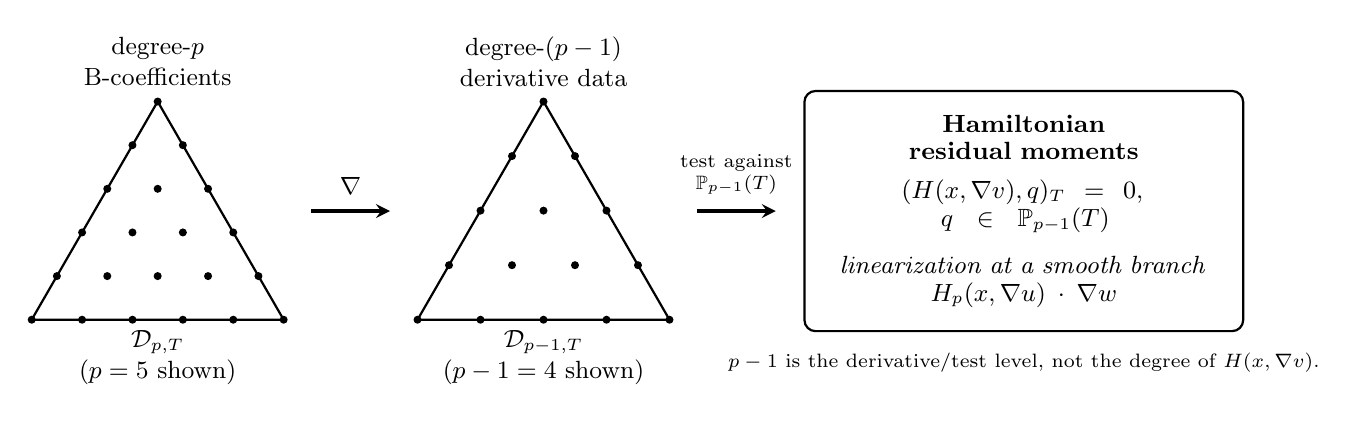
\begin{tikzpicture}[x=1cm,y=1cm,>=stealth,font=\small]
% degree-p Bernstein data
\begin{scope}
  \draw[thick] (0,0)--(3.2,0)--(1.6,2.771)--cycle;
  \foreach \i in {0,...,5}{\foreach \j in {0,...,5}{\pgfmathtruncatemacro{\s}{\i+\j}\ifnum\s<6
    \pgfmathsetmacro{\x}{3.2*\i/5 + 1.6*\j/5}\pgfmathsetmacro{\y}{2.771*\j/5}
    \fill (\x,\y) circle (1.45pt);\fi}}
  \node[align=center] at (1.6,3.28) {degree-$p$\\B-coefficients};
  \node[align=center] at (1.6,-0.48) {$\mathcal D_{p,T}$\\($p=5$ shown)};
\end{scope}

% exact derivative map
\draw[->,very thick] (3.55,1.38)--(4.55,1.38)
  node[midway,above=2pt] {$\nabla$};

% degree-(p-1) derivative data
\begin{scope}[xshift=4.9cm]
  \draw[thick] (0,0)--(3.2,0)--(1.6,2.771)--cycle;
  \foreach \i in {0,...,4}{\foreach \j in {0,...,4}{\pgfmathtruncatemacro{\s}{\i+\j}\ifnum\s<5
    \pgfmathsetmacro{\x}{3.2*\i/4 + 1.6*\j/4}\pgfmathsetmacro{\y}{2.771*\j/4}
    \fill (\x,\y) circle (1.45pt);\fi}}
  \node[align=center] at (1.6,3.28) {degree-$(p-1)$\\derivative data};
  \node[align=center] at (1.6,-0.48) {$\mathcal D_{p-1,T}$\\($p-1=4$ shown)};
\end{scope}

% nonlinear residual moments
\draw[->,very thick] (8.45,1.38)--(9.45,1.38)
  node[midway,above=2pt,align=center,font=\scriptsize] {test against\\$\PP_{p-1}(T)$};

\node[draw,rounded corners,thick,align=center,text width=5.15cm,
      minimum height=3.05cm,inner sep=6pt,anchor=west] (HJ) at (9.8,1.38)
{\textbf{Hamiltonian}\\[-1pt]\textbf{residual moments}\\[3pt]
$\displaystyle (H(x,\nabla v),q)_T=0,$\\[-1pt]
$\displaystyle q\in\PP_{p-1}(T)$\\[6pt]
\textit{linearization at a smooth branch}\\[-1pt]
$\displaystyle H_p(x,\nabla u)\cdot\nabla w$};
\node[font=\scriptsize,anchor=north] at ([yshift=-4pt]HJ.south)
{$p-1$ is the derivative/test level, not the degree of $H(x,\nabla v)$.};
\end{tikzpicture}
\caption{Bernstein $p\to p-1$ mechanism for a stationary Hamilton--Jacobi equation.  The gradient of a degree-$p$ B-form is an exact degree-$(p-1)$ B-form.  The nonlinear Hamiltonian need not have degree $p-1$; the degree shift belongs to the derivative data, the moment test level, and the first-order characteristic linearization.}
\label{fig:pminus1}
\end{figure}

\subsection{Global $C^0$ assembly first}
Let $\Delta$ be a conforming triangulation of $\Omega$.  We use the standard continuous spline space
\[
 S_p^0(\Delta)=\{v\in C^0(\overline\Omega):v|_T\in\PP_p(T)\text{ for every }T\in\Delta\}.
\]
In B-form, continuity across an edge is expressed directly through shared edge coefficients~\cite{LaiSchumaker2007}: the coefficients whose domain points lie on that edge are shared.  Our implementation assigns a single global index to each vertex and edge B-coefficient and separate indices only to triangle-interior coefficients.  Hence continuity is algebraic and exact before the PDE residual is ever evaluated.

This ordering is central to the method.  If one first constructs independent local nonlinear manifolds and couples them later, the resulting analysis is not an analysis of a conforming approximation space.  Here the unknown vector is always a coordinate vector of $S_p^0(\Delta)$ (or of its affine subspace satisfying prescribed trace data).

\section{Local nonlinear quasi-Trefftz structure}\label{sec:local}
Assume first that $H=H(x,p)$ is $C^2$ with respect to the momentum variable on a neighborhood of the exact gradient range.  For one triangle $T$, define the degree-$p$ Hamilton--Jacobi moment manifold
\begin{equation}\label{eq:Mp}
 \mathcal M_p^H(T)=\left\{v\in\PP_p(T):(H(x,\grad v),q)_T=0\quad\forall q\in\PP_{p-1}(T)\right\}.
\end{equation}
This is generally a nonlinear algebraic or smooth finite-dimensional manifold, not a vector space.  In the eikonal specialization~\eqref{eq:Heik}, it reduces to the manifold used in the original eikonal construction.

\subsection{Linearization and characteristic transport}
Let $u$ be a smooth exact branch and set
\begin{equation}\label{eq:achar}
 a(x)=H_p(x,\grad u(x)).
\end{equation}
The Fr\'echet derivative of the Hamiltonian residual is
\begin{equation}\label{eq:linearization}
 D\mathcal H(u)[w]=a(x)\cdot\grad w.
\end{equation}
Thus $a$ is the characteristic transport field.  For the eikonal Hamiltonian~\eqref{eq:Heik}, $a=\grad u$.  For the anisotropic quadratic Hamiltonian $H(x,p)=\tfrac12p^TA(x)p-f(x)$, one has $a=A(x)\grad u$.

Choose an edge $e\subset\partial T$ and let $\lambda_e$ denote the barycentric coordinate that vanishes on $e$.  The associated deep space is
\begin{equation}\label{eq:deep}
 W_{p,T}=\lambda_e\PP_{p-1}(T),\qquad \dim W_{p,T}=\dim\PP_{p-1}(T)=\frac{p(p+1)}2.
\end{equation}
Its functions vanish on $e$ and are the polynomial directions that can be determined by transport from a transverse trace.

\begin{assumption}[Characteristic transversality]\label{ass:trans}
There is an edge $e$ and a number $\beta>0$ such that
\begin{equation}\label{eq:trans}
 \abs{a(x)\cdot\nu_e}\ge\beta\quad\text{on }T,
\end{equation}
where $\nu_e$ is a fixed unit normal to $e$.  Moreover the characteristic field varies moderately on $T$:
\begin{equation}\label{eq:curv}
 h_T\norm{\grad a}_{L^\infty(T)}\le c_0\beta
\end{equation}
for a sufficiently small constant $c_0$ depending only on shape regularity and the fixed polynomial degree.
\end{assumption}

Define $L_{u,T}:W_{p,T}\to\PP_{p-1}(T)'$ by
\begin{equation}\label{eq:Lu}
 \langle L_{u,T}w,q\rangle=(a\cdot\grad w,q)_T.
\end{equation}

\begin{proposition}[Characteristic deep block]\label{prop:block}
Under Assumption~\ref{ass:trans}, $L_{u,T}$ is invertible.  After affine scaling to a shape-regular reference triangle, there is a constant $C$ such that
\begin{equation}\label{eq:blockbound}
 \norm{w}_{0,T}+h_T\abs{w}_{1,T}
 \le C\frac{h_T}{\beta}\norm{L_{u,T}w}_{\PP_{p-1}(T)'},\qquad w\in W_{p,T}.
\end{equation}
\end{proposition}

\begin{proof}
Freeze $a$ at $x_T\in T$, writing $a_T=a(x_T)$.  For $w\in W_{p,T}$, $a_T\cdot\grad w\in\PP_{p-1}(T)$.  If all of its moments against $\PP_{p-1}(T)$ vanish, then $a_T\cdot\grad w=0$ pointwise.  Since $w|_e=0$ and $a_T$ is transverse to $e$, $w$ is zero along every straight characteristic entering through $e$, hence $w=0$.  The frozen square map is therefore invertible.  Affine scaling gives the factor $h_T/|a_T\cdot\nu_e|$.  The variable-field perturbation satisfies
\[
 \norm{(a-a_T)\cdot\grad w}_{0,T}
 \le Ch_T\norm{\grad a}_{L^\infty(T)}\abs{w}_{1,T}.
\]
Assumption~\ref{ass:trans} makes this a sufficiently small perturbation of the frozen transport block.  A Neumann-series argument gives the result.
\end{proof}

\begin{proposition}[Trace-sized tangent nullity]\label{prop:dim}
Suppose $u\in\mathcal M_p^H(T)$ is a regular point of the moment map, so its Jacobian has full row rank $\dim\PP_{p-1}(T)$.  Then
\begin{equation}\label{eq:dim}
 \dim T_u\mathcal M_p^H(T)=\dim\PP_p(T)-\dim\PP_{p-1}(T)=p+1.
\end{equation}
\end{proposition}
\begin{proof}
Apply rank--nullity to the Jacobian of the moment map.  Proposition~\ref{prop:block} supplies a geometrically meaningful full-rank block under characteristic transversality.
\end{proof}

The $p+1$ count is a \emph{single-triangle} tangent dimension.  It must not be confused with the dimension of an already assembled multi-element $C^0$ manifold.  For example, a four-triangle fan with one interior vertex has
\[
 \dim S_p^0(\Delta_P)=5+8(p-1)+4\frac{(p-1)(p-2)}2=2p^2+2p+1,
\]
whereas four complete degree-$(p-1)$ moment blocks contain $2p(p+1)$ rows.  The formal dimension difference is therefore one, not $p+1$.  This simple count is the reason that the global reduction below is performed \emph{after} $C^0$ assembly and uses a rank-revealing independent moment block; see Section~
ef{sec:global}.  Shared-edge coefficients are never removed separately on the two neighboring elements: each such coefficient has one global index and, if condensed, remains a single dependent $C^0$ coefficient.

\begin{remark}[Hamiltonians depending explicitly on $u$]\label{rem:udep}
For a proper stationary equation with explicit solution dependence, linearization of
\[
 H(x,u,\grad u)=0
\]
gives
\[
 H_p(x,u,\grad u)\cdot\grad w+H_u(x,u,\grad u)w.
\]
The Bernstein derivative map and the $p-1$ test level are unchanged.  The zero-order term is a lower-order perturbation of the characteristic block; the proof above extends whenever its scaled size, together with the variation of $H_p$, remains below the transverse transport bound.  To keep the main estimates transparent, the remainder of the analysis is written for $H(x,p)$.
\end{remark}

\section{Conforming embedded quasi-Trefftz reduction}\label{sec:global}
The global discretization is now defined as an actual equation-adapted reduction of the already assembled conforming parent space.  This distinction is essential: minimizing the complete moment residual over $S_p^0(\Delta)$ would be a nonlinear least-squares residual method, whereas the construction below places the trial state on an implicit quasi-Trefftz manifold before any remaining consistency quantity is measured.

Let $c\in\mathbb R^{N_h}$ be the coefficient vector of $S_p^0(\Delta)$.  Because the assembly of Section~\ref{sec:bb} has already identified every shared-edge B-coefficient, every value of $c$ represents a globally $C^0$ function.  Split the coordinates as
\begin{equation}\label{eq:trace-deep-split}
 c=(t,d),
\end{equation}
where $t\in\mathbb R^{N_t}$ contains the retained trace coordinates and $d\in\mathbb R^{N_d}$ contains the coordinates to be condensed, with $N_t+N_d=N_h$.  In the computations below, $t$ consists of the exterior-boundary Bernstein coefficients for Dirichlet branch tests; source-only factorizations retain the prescribed source coordinate instead.  More generally, for first-order problems with mixed inflow/outflow boundary conditions, the inflow Bernstein trace belongs to $t$ while outflow boundary coefficients may be left in $d$ and are then determined by the qT equations.  Importantly, coefficients on \emph{interior} mesh edges belong to $d$ only as single globally shared coordinates.  Their condensation therefore cannot break continuity.

For every element $T$ and every $B^{p-1}_\beta\in\PP_{p-1}(T)$ define
\begin{equation}\label{eq:resrow}
 R_{T,\beta}(c)=\int_T H(x,\grad u_h(c))B^{p-1}_\beta\,dx,
\end{equation}
and collect the rows in $R(c)\in\mathbb R^{N_R}$, where
\[
 N_R=|\Delta|\dim\PP_{p-1}(T).
\]
At a branch seed $c_\star$, form the Jacobian with respect to the dependent coordinates,
\[
 J_d(c_\star)=D_dR(c_\star)\in\mathbb R^{N_R\times N_d}.
\]
A rank-revealing QR factorization of $J_d(c_\star)^T$ selects a row set $I\subset\{1,\ldots,N_R\}$ with $|I|=N_d$ such that
\begin{equation}\label{eq:pivotblock}
 A_\star:=D_dR_I(c_\star)\in\mathbb R^{N_d\times N_d}
\end{equation}
is nonsingular.  The \emph{conforming embedded quasi-Trefftz manifold} is then
\begin{equation}\label{eq:globalqtmanifold}
 \mathcal V_{p,h}^{\rm qT}
 =\{u_h(t,d)\in S_p^0(\Delta):R_I(t,d)=0\}.
\end{equation}
Thus quasi-Trefftz is a property of the trial manifold itself, not merely of the objective minimized by the nonlinear solver.  We use ``local qT manifold'' for the elementwise set $\mathcal M_p^H(T)$ and ``global qT manifold'' for the assembled conforming reduction $\mathcal V_{p,h}^{
m qT}$.

\begin{proposition}[Implicit qT condensation]\label{prop:implicitqt}
Suppose $A_\star$ in~\eqref{eq:pivotblock} is nonsingular.  Then there are neighborhoods of $t_\star$ and $d_\star$ and a unique smooth map $D$ such that
\[
 R_I(t,D(t))=0,
 \qquad D(t_\star)=d_\star.
\]
Consequently $\mathcal V_{p,h}^{\rm qT}$ is locally an $N_t$-dimensional manifold contained in $S_p^0(\Delta)$.
\end{proposition}
\begin{proof}
This is the finite-dimensional implicit-function theorem applied to $R_I(t,d)$ with derivative $D_dR_I=A_\star$.
\end{proof}

For prescribed trace data $t=g_h$, the discrete qT branch is obtained from the square nonlinear system
\begin{equation}\label{eq:qtcondense}
 R_I(g_h,d_h)=0,
\end{equation}
not by minimizing all rows of $R$.  Newton updates use the square pivot block $D_dR_I$.  The complementary rows
\begin{equation}\label{eq:consistencydefect}
 \eta_h:=R_{I^c}(g_h,d_h)
\end{equation}
are retained as a consistency defect.  They are useful for assessing how strongly the selected qT manifold also satisfies the unresolved moment directions, but they do not define the trial manifold.

\begin{figure}[tbp]
\centering
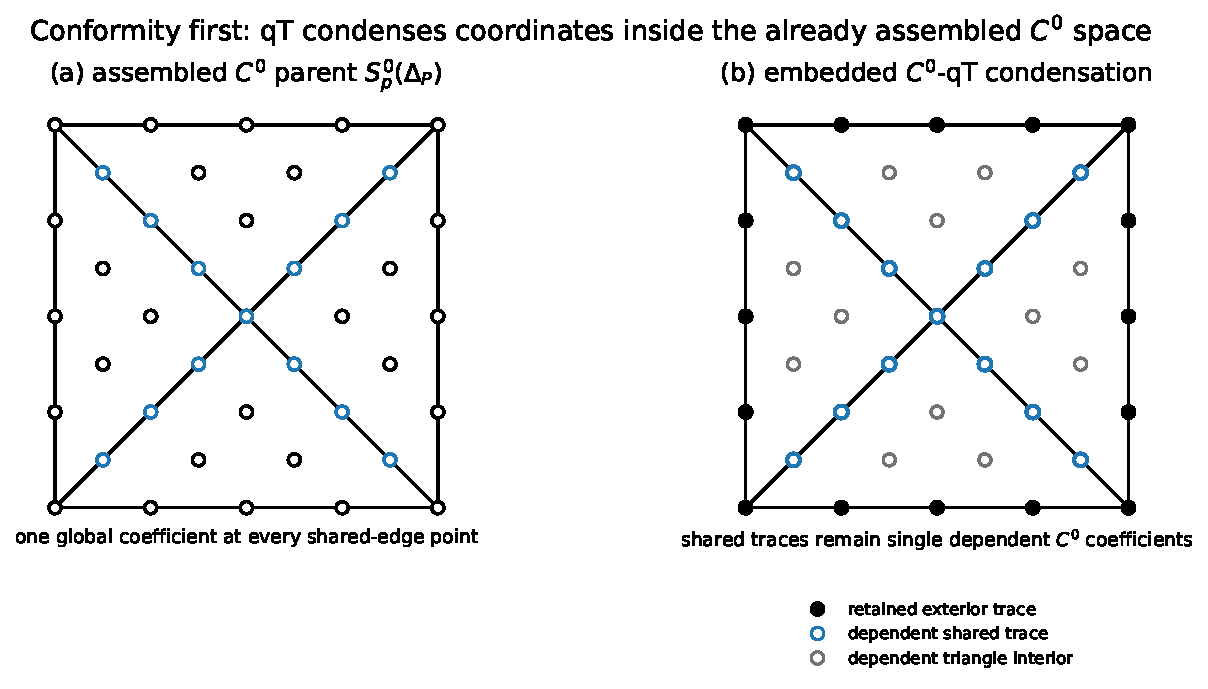
\includegraphics[width=.88\textwidth]{c0_qt_condensation_schematic.pdf}
\caption{Conformity-first embedded qT reduction on a four-triangle patch ($p=4$ shown).  In the assembled parent space (left), every internal-edge domain point already has one shared global coefficient.  In the qT representation (right), exterior trace coordinates are retained, while shared internal-edge and triangle-interior coordinates become dependent variables reconstructed by the selected moment equations.  A dependent shared-edge coefficient is not deleted or set to zero; the same reconstructed coefficient is used by both neighboring triangles.}
\label{fig:c0qtcondensation}
\end{figure}

The distinction in Figure~\ref{fig:c0qtcondensation} is important: qT reduction changes which global coordinates are independent, not the continuity relations of the parent spline.

The analytic Jacobian row is
\begin{equation}\label{eq:jac}
 \frac{\partial R_{T,\beta}}{\partial c_j}
 =\int_T B^{p-1}_\beta\,
 H_p(x,\grad u_h)\cdot\grad\varphi_j\,dx.
\end{equation}
The implementation assembles $J_d$ sparsely, performs the rank-revealing row selection at the branch seed, and then keeps that row set fixed so long as the selected block remains well conditioned.  In practice we monitor $\sigma_{\min}(D_dR_I)$ during Newton iteration; if it drops by more than a prescribed factor relative to $\sigma_{\min}(A_\star)$, the QR selection is recomputed and the defining row set is refreshed.  None of the reported runs required reselection, but the safeguard is part of the algorithmic definition.  The selected square system is solved by sparse Newton steps with backtracking.  Hence no interior or interelement coefficient survives as an independent unknown merely because it was present in the parent polynomial space; however every reconstructed coefficient remains a coefficient of the same globally assembled $C^0$ spline.

\begin{remark}[Why this is different from the earlier residual prototype]\label{rem:lsproto}
The original prototype minimized $\|R(c)\|_2$ over all free coefficients of $S_p^0(\Delta)$.  That calculation is useful as a branch-correction benchmark, and those previously computed application runs are retained below where explicitly identified.  It is not the definition of the qT method.  In the present formulation the selected moment equations~\eqref{eq:qtcondense} are satisfied to nonlinear solver tolerance before the complementary consistency defect~\eqref{eq:consistencydefect} is examined.
\end{remark}

\section{Viscosity solutions and branch selection}\label{sec:viscosity}
Stationary Hamilton--Jacobi equations generally admit nonsmooth solutions even when the Hamiltonian and boundary data are smooth.  The appropriate global solution concept is therefore the viscosity solution~\cite{CrandallIshiiLions1992}.  In the first-order setting considered here, a continuous function $u$ is interpreted through test functions that touch it from above or below: if $\phi\in C^1$ and $u-\phi$ has a local maximum at $x_0$, the subsolution inequality requires
\[
   H(x_0,\grad\phi(x_0))\le 0,
\]
while at a local minimum the supersolution inequality is
\[
   H(x_0,\grad\phi(x_0))\ge 0.
\]
With the appropriate boundary interpretation, comparison principles then identify the physically relevant solution even when classical derivatives fail to exist.  For the eikonal equation this is the first-arrival travel time.

The present $C^0$ quasi-Trefftz formulation is intentionally not a monotone viscosity scheme.  Its defining manifold is built from high-order signed moment equations, and the nonlinear Newton condensation has no positivity or monotonicity structure.  Consequently, the monotonicity hypothesis in the Barles--Souganidis convergence framework~\cite{BarlesSouganidis1991} is not available, and small discrete Hamiltonian residual alone does not identify the viscosity solution.  A different smooth classical branch may also satisfy the Hamiltonian equation to high accuracy.  The approximation theory in Section~\ref{sec:approx} should therefore be read branchwise: it applies on regions where the selected viscosity solution coincides with a sufficiently smooth classical branch and the characteristic field $H_p(x,\grad u)$ satisfies the transversality assumption.

There are two branch-selection mechanisms used in the numerical experiments.  The first is explicit branch construction.  Suppose smooth classical branches $u_1,\ldots,u_m$ are available and the physical selection rule is known.  For first-arrival eikonal problems the viscosity solution is the lower envelope
\begin{equation}\label{eq:visc-min}
   u(x)=\min_{1\le j\le m}u_j(x).
\end{equation}
Each $u_j$ may be approximated with high order by the qT formulation on its smooth region, and the nonsmooth switching set is introduced only by the final minimum.  Section~\ref{sec:two-source} uses exactly this construction for two point sources.  Thus high-order approximation and viscosity selection are separated rather than asking one nonmonotone polynomial solve to perform both tasks.

The second mechanism is causal branch initialization.  For a general first-arrival problem where the relevant branch is not known analytically, we first compute a coarse monotone or causal approximation $u_h^{\rm c}$.  Marching, ordered-upwind, and sweeping methods are natural choices because their discrete causality selects the viscosity branch robustly~\cite{Sethian1996,SethianVladimirsky2003,Zhao2005}.  The qT solve is then initialized from $u_h^{\rm c}$ and used only as a high-order correction of that selected branch.  Schematically,
\begin{equation}\label{eq:causal-qt}
   \text{causal viscosity selector}
   \;\longrightarrow\;
   \text{smooth branch initialization}
   \;\longrightarrow\;
   C^0\text{-qT correction}.
\end{equation}
This is the architecture used for Marmousi in Section~\ref{sec:marmousi}.  There the causal computation is deliberately much coarser than the reference grid, so the subsequent improvement measures the effect of the qT correction rather than merely reproducing a fine-grid causal solution.

This distinction also explains the error behavior near shocks, branch-switching curves, and caustics.  Away from the viscosity singular set, the solution is locally classical and the high-order branch approximation estimates may apply.  Across the singular set, global smoothness is lost and no spectral-in-$p$ behavior should be expected.  Moreover, continuing to reduce the nonmonotone moment residual can move the discrete state away from the viscosity branch even while $\|R(z)\|_2$ decreases.  For this reason the causal experiments use limited inexact nonlinear correction as a branch-preserving regularization.  The resulting method is therefore best viewed as a high-order local corrector for a viscosity branch selected by separate physical or causal information, not as a stand-alone general-purpose viscosity solver.

The distinction is important for interpreting the results that follow.  Smooth manufactured problems test the embedded qT approximation mechanism itself; the two-source example tests explicit viscosity selection by the envelope~\eqref{eq:visc-min}; Marmousi tests causal selection followed by the retained parent-space branch correction; and the focal experiment tests a known singular factor while remaining branchwise.  None of these experiments is used to claim monotone convergence of the qT formulation to arbitrary viscosity solutions.

\section{Eikonal specialization: point-source and focal factoring}\label{sec:factoring}
For the eikonal Hamiltonian~\eqref{eq:Heik}, suppose the solution contains a known singular phase $T$ and write
\begin{equation}\label{eq:factor}
  u=T+\tau.
\end{equation}
The correction $\tau$ is approximated in $S_p^0(\Delta)$.  Its residual is
\begin{equation}\label{eq:factres}
 F_n(T+\tau)=\frac12\left(\abs{\grad T+\grad\tau}^2-n^2\right),
\end{equation}
and the derivative in a polynomial direction $w$ is
\begin{equation}\label{eq:factlin}
 D_\tau F_n(T+\tau)[w]=(\grad T+\grad\tau)\cdot\grad w=\grad u\cdot\grad w.
\end{equation}
Hence factoring removes the singularity from the polynomial unknown without changing the first-order $p-1$ tangent structure.

For a point source $x_s$ in a smooth isotropic medium, a standard choice is
\[
  T(x)=n(x_s)\abs{x-x_s}.
\]
This follows the same singularity-removal principle as factored sweeping and marching methods~\cite{FomelLuoZhao2009,TreisterHaber2016}.  For the focal experiment in Section~\ref{sec:focal}, the singular factor has the opposite sign, $T=-\abs{x-x_c}$, representing an inward travelling phase whose rays converge at $x_c$.

\section{Approximation and branchwise error analysis}\label{sec:approx}
We first generalize the local approximation result from the quadratic eikonal Hamiltonian to a smooth stationary Hamiltonian.  Let $u$ be a classical solution of~\eqref{eq:HJ} on $T$, assume $u\in H^s(T)\cap W^{2,\infty}(T)$ with $2\le s\le p+1$, and suppose Assumption~\ref{ass:trans} holds.  Assume also that $H$ is $C^2$ in $p$ on a convex neighborhood $\mathcal K$ containing the gradients considered below, with
\begin{equation}\label{eq:Hppbound}
 \sup_{x\in T,\,\xi\in\mathcal K}\norm{H_{pp}(x,\xi)}\le M_H.
\end{equation}

Let $\pi_pu\in\PP_p(T)$ be a polynomial approximant and put $e=\pi_pu-u$.  Taylor's theorem in the momentum variable gives
\begin{equation}\label{eq:taylorH}
 H(x,\grad\pi_pu)
 =a(x)\cdot\grad e
 +\frac12\grad e^T
 H_{pp}(x,\grad u+\theta(x)\grad e)\grad e
\end{equation}
for some $0<\theta(x)<1$.  Consequently
\begin{equation}\label{eq:remainderH}
 \abs{H(x,\grad\pi_pu)-a\cdot\grad e}
 \le \frac{M_H}{2}\abs{\grad e}^2.
\end{equation}
For the eikonal Hamiltonian $H_{pp}=I$, and~\eqref{eq:taylorH} reduces exactly to the familiar linear term $\grad u\cdot\grad e$ plus $\tfrac12|\grad e|^2$.

\begin{theorem}[Local Hamilton--Jacobi quasi-Trefftz approximation]\label{thm:approx}
Under the hypotheses above, for $h_T$ sufficiently small there exists $v_p\in\mathcal M_p^H(T)$ such that
\begin{align}
 \abs{u-v_p}_{1,T}&\le C h_T^{s-1}\abs{u}_{s,T},\label{eq:H1approx}\\
 \norm{u-v_p}_{0,T}&\le C h_T^s\abs{u}_{s,T}.\label{eq:L2approx}
\end{align}
The constant depends on shape regularity, $p$, the transversality ratio, $M_H$, and bounds on the characteristic field, but not on $h_T$.
\end{theorem}

\begin{proof}
Choose $\pi_pu$ with the standard polynomial approximation bounds on a shape-regular triangle~\cite{Ciarlet2002}.  Seek a correction $d\in W_{p,T}$ such that the moment map of $\pi_pu+d$ vanishes.  At $d=0$, the derivative with respect to $d$ is
\[
 w\mapsto \bigl(H_p(x,\grad\pi_pu)\cdot\grad w,\,\cdot\bigr)_T.
\]
Because $\grad\pi_pu$ converges uniformly to $\grad u$ for a smooth branch, this is a small perturbation of the characteristic block in Proposition~\ref{prop:block}.  It is therefore invertible for sufficiently small $h_T$.  The defect at $d=0$ is controlled by~\eqref{eq:taylorH}: its leading term is the transport of the polynomial approximation error and its nonlinear part is quadratic in $\grad e$.  The inverse estimate~\eqref{eq:blockbound}, followed by a finite-dimensional implicit-function/Newton argument, gives a correction whose scaled $L^2$--$H^1$ norm is no larger than the ordinary polynomial approximation error.  Combining the correction with the approximation bounds for $\pi_pu$ proves~\eqref{eq:H1approx}--\eqref{eq:L2approx}.
\end{proof}

\begin{remark}[Local versus global approximation]\label{rem:localglobal}
Theorem~
ef{thm:approx} is an elementwise result.  Independently chosen states $v_p\in\mathcal M_p^H(T)$ do not in general possess matching traces on neighboring triangles, so the theorem does not by itself produce a global conforming approximant.  Global conformity is imposed first through $S_p^0(\Delta)$, and the assembled qT manifold $\mathcal V_{p,h}^{
m qT}$ inherits approximation through a conforming parent approximant together with the nonlinear stability estimate of Theorem~
ef{thm:global}.
\end{remark}

\subsection{Perturbation of the Hamiltonian}
In heterogeneous applications one may construct the local residual with an approximation $H_h$ of $H$.  We denote by $\mathcal M_p^{H_h}(T)$ the moment manifold defined as in~\eqref{eq:Mp} with $H$ replaced by $H_h$.  Let $\pi_pu$ be the polynomial approximant used above and define the moment-level consistency defect
\begin{equation}\label{eq:epsH}
 \varepsilon_{H,T}:=
 \norm{q\mapsto (H_h(x,\grad\pi_pu)-H(x,\grad\pi_pu),q)_T}_{\PP_{p-1}(T)'}.
\end{equation}
The same correction argument gives an element $v_{p,h}\in\mathcal M_p^{H_h}(T)$ satisfying the perturbed estimate
\begin{equation}\label{eq:Hperturb}
 \norm{u-v_{p,h}}_{0,T}+h_T\abs{u-v_{p,h}}_{1,T}
 \le C h_T^s\abs{u}_{s,T}
 +C\frac{h_T}{\beta}\varepsilon_{H,T},
\end{equation}
provided the perturbed characteristic block remains invertible.  This separates approximation of the branch from approximation of the Hamiltonian itself.  In the eikonal experiments the analytic slowness is evaluated directly at quadrature points, so no coefficient-projection term is present.

\subsection{Stability of the implicit qT condensation}
The local approximation theorem describes what the Hamilton--Jacobi moment equations can represent.  The global conforming reduction additionally requires the selected dependent-coordinate block to remain invertible.  Let $c_\star=(t_\star,d_\star)$ be a conforming branch approximant and set
\begin{equation}\label{eq:sigmah}
 \sigma_h=\sigma_{\min}\bigl(D_dR_I(c_\star)\bigr).
\end{equation}

\begin{theorem}[Local stability of the conforming qT map]\label{thm:global}
Assume $\sigma_h>0$ and that $D_dR_I$ is Lipschitz in a ball of radius $\rho$ about $c_\star$, with Lipschitz constant $L_h$ satisfying $L_h\rho\le\sigma_h/2$.  Fix trace coordinates $t$ in this ball.  If $d_h=D(t)$ is the qT-condensed coordinate vector from Proposition~\ref{prop:implicitqt}, then
\begin{equation}\label{eq:globalbound}
 \norm{d_h-d_\star}
 \le \frac{2}{\sigma_h}\norm{R_I(t,d_\star)}.
\end{equation}
Consequently the qT reduction preserves the approximation order of a conforming parent approximant whenever the selected moment defect has the same order and $\sigma_h$ remains uniformly bounded away from zero in the chosen scaling.
\end{theorem}
\begin{proof}
For fixed $t$, the fundamental theorem of calculus gives
\[
 R_I(t,d)-R_I(t,d_\star)
 =D_dR_I(c_\star)(d-d_\star)+E(d)(d-d_\star),
\]
with $\norm{E(d)}\le L_h\rho\le\sigma_h/2$.  Hence
\[
 \norm{R_I(t,d)-R_I(t,d_\star)}
 \ge \frac{\sigma_h}{2}\norm{d-d_\star}.
\]
Set $d=d_h$ and use $R_I(t,d_h)=0$ to obtain~\eqref{eq:globalbound}.
\end{proof}

Theorem~\ref{thm:global} is deliberately a branchwise statement.  It concerns the stability of the implicit qT condensation, not monotone convergence to an arbitrary viscosity solution.  The selected singular value $\sigma_h$ is also a practical conditioning quantity for the nonlinear static condensation.

\section{Numerical experiments}\label{sec:numerics}
All computations are in double precision.  Unless stated otherwise, relative $L^2$ error means $\norm{u-u_h}_{0}/\norm{u}_{0}$ with $\norm{\cdot}_{0}:=\norm{\cdot}_{L^2(\Omega)}$, and relative $H^1$ error means the seminorm ratio $\abs{u-u_h}_{1}/\abs{u}_{1}$.  For a residual vector with $N_R$ rows, ``residual RMS'' means $\norm{R}_{2}/\sqrt{N_R}$.  Triangle integrals use tensor Gauss rules on a Duffy map with order at least $\max(8,2p+3)$, increased for the nonpolynomial Hamiltonian test.  Analytic Jacobians are assembled from~\eqref{eq:jac}.  Unless a test explicitly studies inflow or source-only data, exact boundary traces are imposed in Bernstein form.

\subsection{Computational protocol and odd-degree continuation}
All degree sweeps in this section use the single sequence
\begin{equation}\label{eq:odddegrees}
  p=3,5,7,9,11,13.
\end{equation}
Even degrees are mathematically admissible; restricting the reported sweeps to one parity gives a consistent six-point sequence and avoids interleaving preasymptotic parity effects in the plots.  Every convergence graph therefore contains at least six computed points.  Mesh sweeps likewise contain six levels.

The core qT experiments below use the implicit condensation of Section~\ref{sec:global}: batched element kernels, direct sparse assembly of the analytic Jacobian, one-time rank-revealing selection of the defining moment block, and sparse Newton solution of the dependent conforming coordinates.  Exact Bernstein degree elevation remains available for continuation in $p$.  Selected qT moment rows are reported separately from the complementary consistency defect.  The Marmousi and several first-arrival stress tests retain the earlier full-residual Gauss--Newton/LSMR branch-correction prototype, and are explicitly identified as hybrid branch-correction experiments rather than as evidence for the reduced qT manifold.  We use DOF to mean degree of freedom and DOFs for its plural.


\subsection{$C^0$ parent space versus $C^0$ quasi-Trefftz reduction}\label{sec:c0qtcompare}
The first experiment isolates the principal question of the paper: whether imposing the Hamilton--Jacobi moment structure removes PDE-incompatible polynomial directions without destroying the approximation quality of the globally conforming parent space.  We use a genuinely two-dimensional rotating-anisotropy Hamiltonian
\begin{equation}\label{eq:rotanis}
 H(x,p)=\frac12 p^T A(x)p-f(x),\qquad
 A(x)=R(\theta(x))
 \begin{pmatrix}1&0\\0&\rho(x)\end{pmatrix}R(\theta(x))^T,
\end{equation}
where the planar rotation matrix is
\[
 R(\vartheta):=
 \begin{pmatrix}
  \cos\vartheta & -\sin\vartheta\\
  \sin\vartheta & \cos\vartheta
 \end{pmatrix},
\]
and
\[
 \theta(x,y)=0.35\sin(\pi x)\cos(\pi y),\qquad
 \rho(x,y)=3+0.5\sin(\pi x)\sin(\pi y).
\]
and $f$ is manufactured from the smooth exact phase
\begin{equation}\label{eq:rotanisphase}
 u=x+0.32y+0.055\sin(2\pi x)\sin(\pi y)
   +0.025\sin(\pi x)\cos(2\pi y).
\end{equation}
Thus both the characteristic direction and the principal axes of the Hamiltonian rotate through the domain.

For each mesh and degree we first compute the $L^2$ projection of~\eqref{eq:rotanisphase} into the full parent space $S_p^0(\Delta)$, with the exact boundary trace imposed in Bernstein form.  Starting from exactly that coefficient vector, we construct the embedded qT manifold~\eqref{eq:globalqtmanifold}: the exterior trace coefficients are retained and a rank-revealing row subset of the degree-$(p-1)$ moment map is solved exactly for every remaining globally assembled $C^0$ coefficient.  Thus the qT state is obtained by nonlinear static condensation, not by residual minimization.  Shared interior-edge coefficients are dependent coordinates of the same global $C^0$ vector and remain single-valued throughout.

\begin{table}[t]
\centering
\small
\caption{Full $C^0$ parent approximation versus the embedded $C^0$-qT reduction for the rotating-anisotropy problem on 32 triangles.  $N_h$ is the parent dimension and $N_t$ the retained boundary-trace dimension before the trace values are prescribed.  The selected qT moments are solved to roundoff.}
\label{tab:c0qtcompare}
\begin{tabular}{rrrrrrr}
\toprule
$p$ & $N_h$ & $N_t$ & full $C^0$ rel. $L^2$ & qT rel. $L^2$ & qT/full & selected RMS\\
\midrule
3  & 169  & 48  & $1.29\times10^{-4}$ & $3.84\times10^{-4}$ & 2.99 & $2.4\times10^{-17}$\\
5  & 441  & 80  & $1.11\times10^{-6}$ & $3.20\times10^{-6}$ & 2.89 & $3.0\times10^{-15}$\\
7  & 841  & 112 & $5.68\times10^{-9}$ & $1.76\times10^{-8}$ & 3.09 & $4.5\times10^{-15}$\\
9  & 1369 & 144 & $1.92\times10^{-11}$ & $5.58\times10^{-11}$ & 2.91 & $4.8\times10^{-19}$\\
11 & 2025 & 176 & $4.33\times10^{-13}$ & $1.51\times10^{-13}$ & 0.35 & $3.2\times10^{-19}$\\
13 & 2809 & 208 & $1.73\times10^{-12}$ & $8.25\times10^{-13}$ & 0.48 & $2.3\times10^{-19}$\\
\bottomrule
\end{tabular}
\end{table}

Figure~\ref{fig:c0qtcompare} gives both the six-point degree sweep and a six-level $h$-sweep at fixed $p=7$.  The defining selected moments are reduced to approximately $10^{-15}$--$10^{-19}$ RMS, so the computed states lie on the selected qT manifold to floating-point accuracy.  The complementary moment rows are not used to define the trial manifold; on the $p$-sweep their RMS falls from $1.53\times10^{-5}$ at $p=3$ to $2.74\times10^{-17}$ at $p=13$.  Before the roundoff floor, the qT $L^2$ error remains within about a factor three of the full $C^0$ best approximation while retaining the same high-order trend.  At $p=7$ the globally assembled parent has 841 coordinates, whereas the implicit qT manifold is parameterized by 112 exterior trace coordinates before those trace values are prescribed.  This is direct numerical evidence of an actual equation-adapted reduction, rather than merely a smaller residual obtained in the unreduced parent space.

\begin{figure}[tbp]
\centering
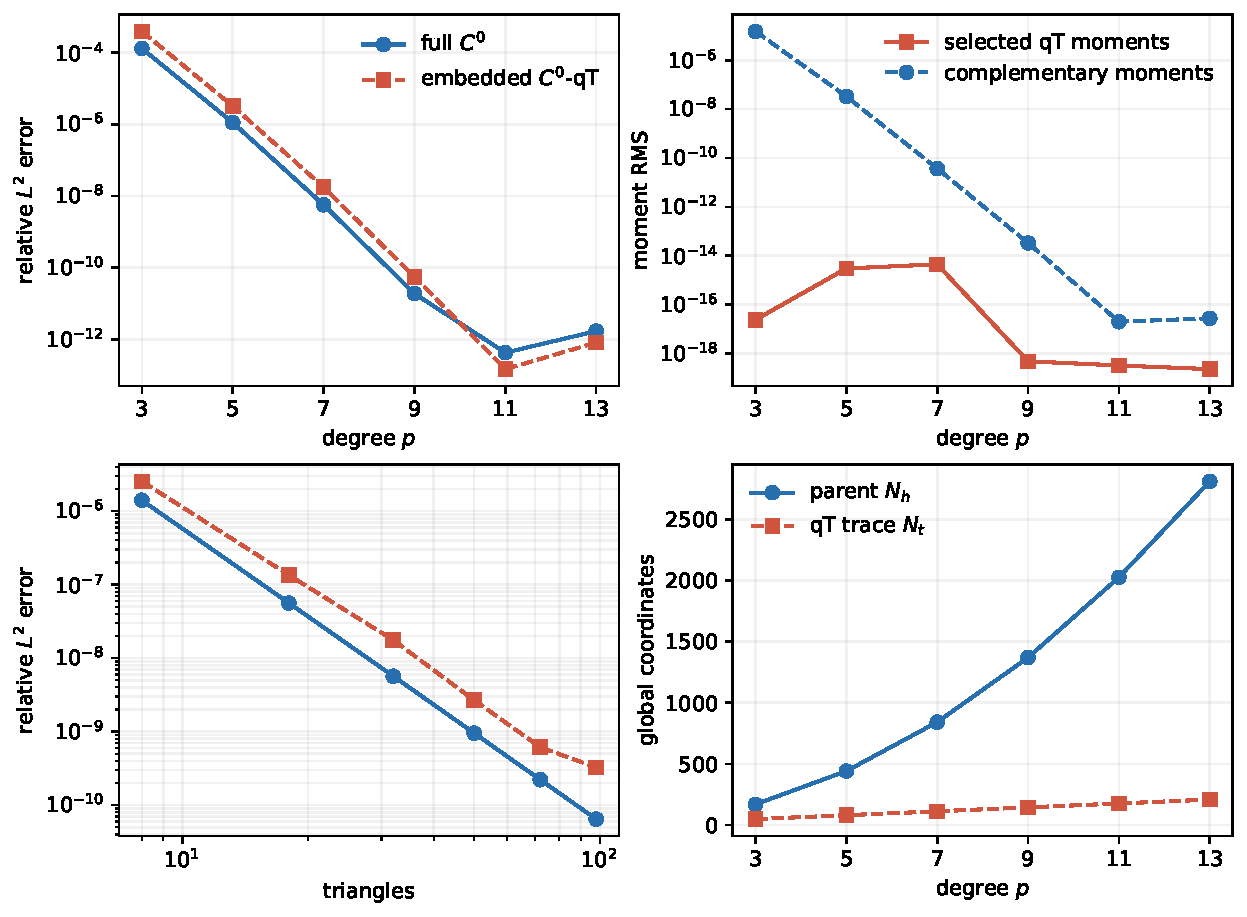
\includegraphics[width=.82\textwidth]{c0_qt_first_experiment.pdf}
\caption{Full $C^0$ parent space versus the embedded $C^0$-qT reduction.  Top left: degree convergence.  Top right: defining selected-moment RMS, showing that the qT constraints are solved to roundoff.  Bottom left: six-level $h$-sweep at $p=7$.  Bottom right: parent dimension versus retained trace dimension.}
\label{fig:c0qtcompare}
\end{figure}

\subsection{Two non-eikonal Hamiltonians}\label{sec:generalHJnum}
Before turning to the eikonal equation, we verify that the construction is not tied to the quadratic Euclidean Hamiltonian.  On the unit square and an 18-triangle mesh, the first test uses
\begin{equation}\label{eq:anisHJ}
 H_2(x,p)=\frac12p^TA(x)p-f_2(x),
\end{equation}
where, for $x=(x_1,x_2)^T$,
\[
 A(x)=\begin{pmatrix}
 1.10+0.18x_1 & 0.10+0.04\sin(\pi x_1)\sin(\pi x_2)\\
 0.10+0.04\sin(\pi x_1)\sin(\pi x_2) & 0.85+0.12x_2
 \end{pmatrix},
\]
which is smooth and symmetric positive definite on the unit square, and $f_2$ is manufactured from the exact phase
\[
 u_2=x+0.30y+0.055\sin(\pi x)\sin(\pi y).
\]
The characteristic velocity is $H_{2,p}=A(x)p$.  The second test is genuinely nonquadratic:
\begin{equation}\label{eq:quarticHJ}
 H_4(x,p)=\frac14(p_1^4+p_2^4)+\frac{0.35}{2}|p|^2-f_4(x),
\end{equation}
with $f_4$ manufactured from
\[
 u_4=x+0.22y+0.045\sin(\pi x)\sin(\pi y).
\]
Here $H_{4,p}=(p_1^3+0.35p_1,p_2^3+0.35p_2)^T$, so the characteristic field is nonlinear in the discrete gradient.

Table~\ref{tab:generalHJ} shows the six-degree embedded-qT sweep.  For both Hamiltonians the defining moment block is solved essentially to roundoff and the complementary residual decays rapidly with $p$.  The anisotropic problem reaches $4.21\times10^{-14}$ relative $L^2$ error at $p=11$ before roundoff amplification at $p=13$; the quartic problem behaves similarly, reaching $5.42\times10^{-14}$ at $p=11$.  Thus the nonlinear qT condensation is not tied to the Euclidean eikonal Hamiltonian.

\begin{table}[t]
\centering
\caption{Embedded $C^0$-qT tests for two non-eikonal stationary Hamilton--Jacobi equations on 18 triangles.  The residual column is the RMS of the selected defining qT moments; the complementary rows are not used to define the manifold.}
\label{tab:generalHJ}
\begin{tabular}{llrrrr}
\toprule
Hamiltonian & $p$ & relative $L^2$ & relative $H^1$ & selected RMS & time (s)\\
\midrule
anisotropic quadratic &3 &$1.14\times10^{-4}$&$2.33\times10^{-3}$&$1.75\times10^{-18}$&0.004\\
&5 &$1.32\times10^{-6}$&$3.74\times10^{-5}$&$7.89\times10^{-18}$&0.027\\
&7 &$5.83\times10^{-9}$&$2.41\times10^{-7}$&$1.11\times10^{-16}$&0.009\\
&9 &$1.83\times10^{-11}$&$9.54\times10^{-10}$&$3.72\times10^{-19}$&0.022\\
&11&$4.21\times10^{-14}$&$2.80\times10^{-12}$&$2.51\times10^{-19}$&0.067\\
&13&$1.16\times10^{-12}$&$9.20\times10^{-11}$&$2.26\times10^{-19}$&0.088\\
\midrule
quartic convex &3 &$1.31\times10^{-4}$&$2.10\times10^{-3}$&$3.07\times10^{-18}$&0.004\\
&5 &$9.04\times10^{-7}$&$2.63\times10^{-5}$&$5.71\times10^{-18}$&0.007\\
&7 &$8.12\times10^{-9}$&$3.72\times10^{-7}$&$1.78\times10^{-16}$&0.008\\
&9 &$1.23\times10^{-11}$&$9.64\times10^{-10}$&$2.99\times10^{-19}$&0.021\\
&11&$5.42\times10^{-14}$&$4.90\times10^{-12}$&$2.63\times10^{-19}$&0.066\\
&13&$6.31\times10^{-13}$&$9.00\times10^{-11}$&$1.91\times10^{-19}$&0.081\\
\bottomrule
\end{tabular}
\end{table}

\subsection{Eikonal equation: exact polynomial recovery}
We begin with
\[
 u(x,y)=x+0.35y+0.08xy,
 \qquad n(x,y)=\abs{\grad u(x,y)}.
\]
On a $2\times2$ structured cell grid (eight triangles), this exact quadratic solution lies in every reported parent space.  Table~\ref{tab:poly} shows that the embedded qT condensation recovers it to the expected floating-point/conditioning floor over the odd-degree sequence.  The defining selected moments remain at or near roundoff, while all shared-edge coefficients remain single global $C^0$ coordinates.

\begin{table}[t]
\centering
\caption{Exact polynomial recovery by the embedded $C^0$-qT reduction on eight triangles.}
\label{tab:poly}
\begin{tabular}{rrrrr}
\toprule
$p$ & global $C^0$ DOFs & relative $L^2$ & relative $H^1$ & selected RMS\\
\midrule
3  & 49  & $7.07\times10^{-16}$ & $1.17\times10^{-14}$ & $1.28\times10^{-16}$\\
5  & 121 & $2.71\times10^{-15}$ & $8.56\times10^{-14}$ & $1.89\times10^{-16}$\\
7  & 225 & $1.27\times10^{-14}$ & $6.12\times10^{-13}$ & $5.16\times10^{-16}$\\
9  & 361 & $6.23\times10^{-14}$ & $4.49\times10^{-12}$ & $2.24\times10^{-15}$\\
11 & 529 & $3.22\times10^{-13}$ & $3.22\times10^{-11}$ & $7.60\times10^{-15}$\\
13 & 729 & $2.04\times10^{-12}$ & $1.24\times10^{-10}$ & $2.89\times10^{-19}$\\
\bottomrule
\end{tabular}
\end{table}

\subsection{Smooth branch: degree and mesh convergence}
The nonpolynomial manufactured phase is
\begin{equation}\label{eq:smoothphase}
 u(x,y)=x+0.35y+0.06\sin(\pi x)\sin(\pi y),
 \qquad n=\abs{\grad u}.
\end{equation}
Its $x$-characteristic component remains positive throughout the unit square.  On 18 triangles, the embedded qT relative $L^2$ error decreases from $1.39\times10^{-4}$ at $p=3$ to $1.12\times10^{-6}$ at $p=5$, $5.77\times10^{-9}$ at $p=7$, and $5.53\times10^{-14}$ at $p=11$ before the conditioning floor is reached.  The corresponding relative $H^1$ error reaches $3.76\times10^{-12}$ at $p=11$.

Figure~\ref{fig:smoothconv} shows all six odd degrees and a six-level mesh sweep at fixed $p=5$.  In the mesh sweep, refinement from 8 to 98 triangles reduces the relative $L^2$ error from $2.22\times10^{-6}$ to $1.89\times10^{-8}$ and the relative $H^1$ error from $4.05\times10^{-5}$ to $1.18\times10^{-6}$.

\begin{figure}[tbp]
\centering
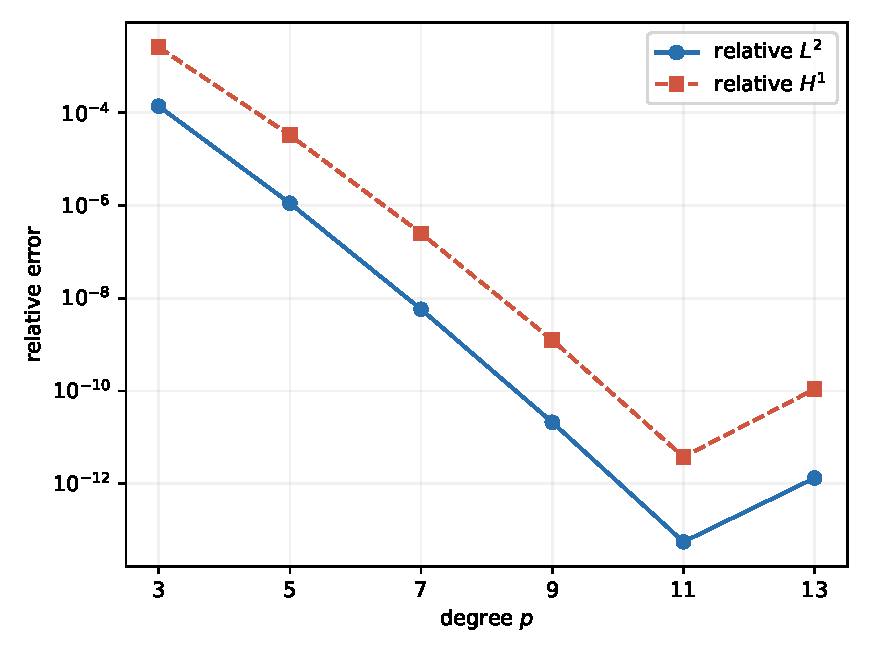
\includegraphics[width=.47\textwidth]{smooth_p_convergence.pdf}\hfill
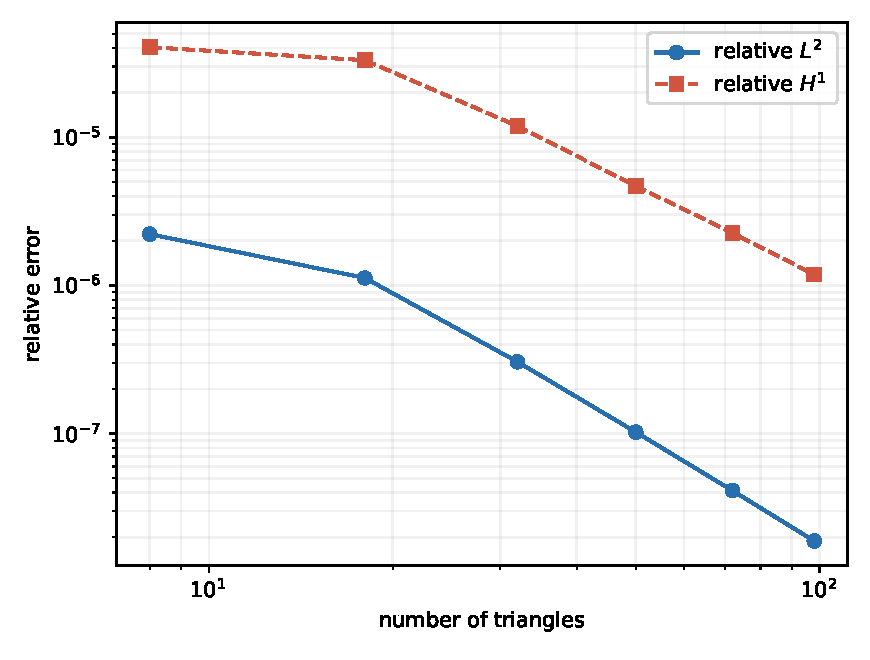
\includegraphics[width=.47\textwidth]{smooth_h_convergence.pdf}
\caption{Smooth manufactured branch. Left: odd-degree refinement $p=3,5,7,9,11,13$ on 18 triangles. Right: six mesh levels at fixed $p=5$.}
\label{fig:smoothconv}
\end{figure}

For the same phase at $p=5$ on 18 triangles, prescribing only the inflow trace on $x=0$ gives relative errors $4.67\times10^{-4}$ in $L^2$ and $3.60\times10^{-3}$ in $H^1$.  This is less accurate than the full-trace validation problem but demonstrates that the assembled nonlinear moment system is not tied to full Dirichlet data.

\subsection{Strongly heterogeneous stratified medium}\label{sec:strat}
We next use the smooth slowness
\begin{equation}\label{eq:stratslow}
 n(y)=1.08+0.42\exp\!\left[-\left(\frac{y-0.58}{0.16}\right)^2\right]
 -0.12\exp\!\left[-\left(\frac{y-0.22}{0.11}\right)^2\right],
\end{equation}
with exact single-arrival phase
\begin{equation}\label{eq:stratphase}
 u(x,y)=\alpha x+\phi(y),\qquad
 \phi'(y)=\sqrt{n(y)^2-\alpha^2},\qquad \phi(0)=0,\qquad \alpha=0.8.
\end{equation}
The conserved horizontal slowness component $\alpha$ gives the standard characteristic/Snell-law structure of stratified geometrical optics~\cite{EngquistRunborg2003,Runborg2007}.  Figure~\ref{fig:strat} shows the computed $p=5$ solution on 32 triangles.

\begin{figure}[tbp]
\centering
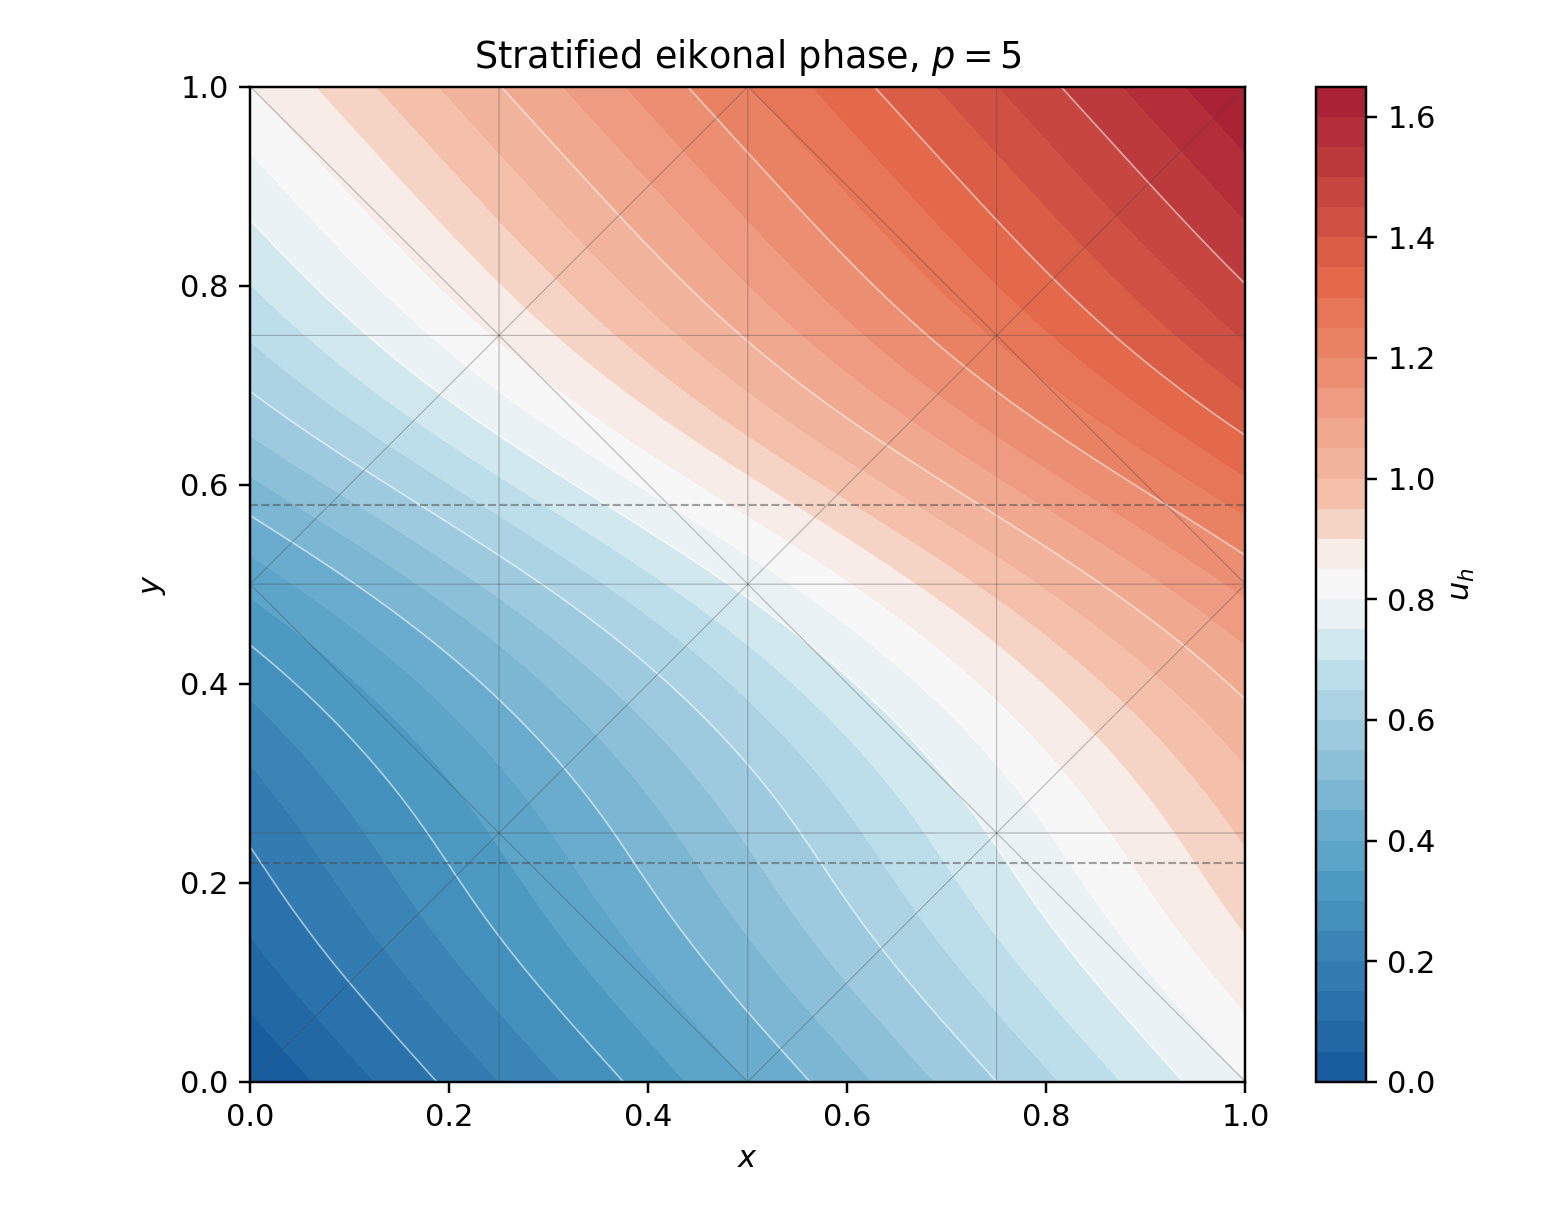
\includegraphics[width=.62\textwidth]{stratified_p5_solution.png}
\caption{Computed degree-$5$ phase in the heterogeneous stratified medium~\eqref{eq:stratslow}.  The solution bends across the slow and fast layers while retaining global $C^0$ continuity.}
\label{fig:strat}
\end{figure}

At $p=5$, a six-level sweep from 8 to 98 triangles reduces the relative $L^2$ error from $4.69\times10^{-4}$ to $1.01\times10^{-6}$ and the relative $H^1$ error from $1.03\times10^{-2}$ to $8.00\times10^{-5}$.  The residual RMS decreases from $2.53\times10^{-6}$ to $1.33\times10^{-9}$, and all six nonlinear solves satisfy the stopping criterion.

\subsection{Benchmark against factored fast marching}\label{sec:thbench}
To place the branchwise Bernstein construction against an established point-source method, we reproduce the first two-dimensional analytic medium of Treister and Haber~\cite{TreisterHaber2016}.  On
\[
 \Omega=[0,4]\times[0,8],\qquad x_s=(0,4),\qquad a_{\rm TH}=-0.4,\qquad s_0=2,
\]
the squared slowness is
\begin{equation}\label{eq:TH1}
 n(x)^2=s_0^2+2a_{\rm TH}(x_1-x_{s,1}).
\end{equation}
Treister and Haber give the corresponding exact travel time in closed form and use it to assess first- and second-order factored fast marching.  We use the same analytic travel time and medium in the error evaluation.

For this comparison we use their multiplicative factorization
\[
 u(x)=r(x)\psi(x),\qquad r(x)=|x-x_s|.
\]
The Bernstein unknown is the smooth factor $\psi_h\in S_p^0(\Delta)$.  No exact outer-boundary trace is supplied: the only prescribed coefficient is the source-limit value $\psi(x_s)=s_0$.  In the notation of Section~\ref{sec:global}, this means $N_t=1$ before prescription, while the table below reports the full parent dimension $N_h$ as a representation-size measure.  All Bernstein rows in Table~\ref{tab:THcompare} use the very coarse fixed mesh $h=1$ and differ only in degree.  At $p=9$ the Bernstein solve is already below the published second-order fast-marching result in both maximum and mean $L^2$ error while using 2701 global coefficients instead of 51681 grid values.  At $p=13$ the maximum error is $1.85\times10^{-6}$ and the mean $L^2$ error is $3.13\times10^{-7}$ with 5565 coefficients.

\begin{table}[t]
\centering
\small
\caption{Treister--Haber 2D test 1: constant gradient of squared slowness.  The fast-marching row is the published second-order result in Table 1 of~\cite{TreisterHaber2016}.  The Bernstein rows use only the factored source value and a fixed $h=1$ mesh.  The DOF column reports the parent $C^0$ dimension $N_h$; in this source-only factorization the retained qT data consist of the single prescribed source value, so $N_t=1$ before prescription and $N_d=N_h-1$.  Timings are included for scale only and are not cross-hardware performance comparisons.}
\label{tab:THcompare}
\begin{tabular}{lrrrrr}
\toprule
method & $h$ & parent DOFs $N_h$ & $\|e\|_{\infty}$ & mean $L^2$ & time (s)\\
\midrule
factored FM, order 2~\cite{TreisterHaber2016} & $1/40$ & 51681 & $9.33\times10^{-5}$ & $9.26\times10^{-6}$ & 0.05\\
BB, $p=3$  & $1$ & 325  & $1.41\times10^{-3}$ & $3.36\times10^{-4}$ & 0.15\\
BB, $p=5$  & $1$ & 861  & $5.93\times10^{-4}$ & $1.57\times10^{-4}$ & 0.19\\
BB, $p=7$  & $1$ & 1653 & $6.81\times10^{-5}$ & $1.94\times10^{-5}$ & 0.70\\
BB, $p=9$  & $1$ & 2701 & $9.70\times10^{-6}$ & $3.38\times10^{-6}$ & 1.50\\
BB, $p=11$ & $1$ & 4005 & $3.58\times10^{-6}$ & $8.45\times10^{-7}$ & 2.98\\
BB, $p=13$ & $1$ & 5565 & $1.85\times10^{-6}$ & $3.13\times10^{-7}$ & 4.85\\
\bottomrule
\end{tabular}
\end{table}

The comparison remains an accuracy/representation benchmark.  For $N$ grid nodes, fast marching is causal, has $O(N\log N)$ complexity, and directly selects the first-arrival viscosity branch.  The Bernstein method instead resolves a selected smooth factored branch with high polynomial order.  The optimized sparse implementation removes the dense-Jacobian bottleneck of the earlier prototype, but it is not intended to compete with fast marching as a large-grid causal solver.

\subsection{Analytic point-source benchmarks}
We use two radial benchmarks from Potter--Cameron~\cite{PotterCameron2019}, with source $x_s=(0,0)$ and radial coordinate $r:=\abs{x-x_s}$:
\[
 u_1(r)=\cos r+r-1,\qquad n_1(r)=1-\sin r,
\]
and
\[
 u_2(r)=\frac12r^2,\qquad n_2(r)=r.
\]
The first has a point-source cusp and is solved with additive factor $T=r$; the second is smooth.  On 32 triangles, the factored $u_1$ problem decreases from relative $L^2$ error $1.19\times10^{-4}$ at $p=3$ to $1.14\times10^{-7}$ at $p=5$, $3.48\times10^{-9}$ at $p=9$, and $6.30\times10^{-10}$ at $p=13$.  The quadratic $u_2$ benchmark is recovered to roundoff for the entire sequence.

A second point-source test places a constant-speed source outside the unit square at $(-0.2,0.5)$, so the phase is smooth inside the domain but retains strong radial curvature.  Table~\ref{tab:point} reports all six odd degrees.  The relative $L^2$ error falls from $1.31\times10^{-4}$ at $p=3$ to $1.77\times10^{-9}$ at $p=13$.

\begin{table}[t]
\centering
\caption{External point source on 32 triangles.  Degree elevation is used between consecutive rows.}
\label{tab:point}
\begin{tabular}{rrrrr}
\toprule
$p$ & relative $L^2$ & relative $H^1$ & residual RMS & time (s)\\
\midrule
3  & $1.31\times10^{-4}$ & $3.59\times10^{-3}$ & $1.40\times10^{-6}$ & 0.043\\
5  & $3.83\times10^{-6}$ & $2.35\times10^{-4}$ & $8.56\times10^{-9}$ & 0.310\\
7  & $1.38\times10^{-7}$ & $1.55\times10^{-5}$ & $6.99\times10^{-11}$ & 1.51\\
9  & $1.04\times10^{-8}$ & $1.63\times10^{-6}$ & $1.71\times10^{-12}$ & 2.13\\
11 & $3.91\times10^{-9}$ & $5.57\times10^{-7}$ & $6.51\times10^{-13}$ & 1.38\\
13 & $1.77\times10^{-9}$ & $2.82\times10^{-7}$ & $3.19\times10^{-13}$ & 1.28\\
\bottomrule
\end{tabular}
\end{table}

\subsection{Linear-speed medium and two-source first arrival}\label{sec:two-source}
For the analytic linear-speed benchmark, let
\[
  \frac1{n(x)}=1+v\cdot x,\qquad v=(0.5,0.25)^T.
\]
For a source $x_i$ the exact travel time is~\cite{PotterCameron2019}
\begin{equation}\label{eq:linear-speed}
 u_i(x)=\frac1{\abs v}\operatorname{arcosh}\!\left(1+
 \frac{n(x_i)n(x)\abs v^2\abs{x-x_i}^2}{2}\right).
\end{equation}
For one source on 32 triangles, the relative $L^2$ error decreases from $1.01\times10^{-5}$ at $p=3$ to $4.29\times10^{-7}$ at $p=5$, $2.65\times10^{-8}$ at $p=9$, and $7.90\times10^{-9}$ at $p=13$.

For two sources at $(0,0)$ and $(0.8,0)$, each smooth factored branch is solved separately at $p=5$ and the physical first arrival is reconstructed as
\[
  u_h(x)=\min\{u_{h,1}(x),u_{h,2}(x)\}.
\]
The relative $L^2$ error is $3.66\times10^{-6}$ and the maximum pointwise error is $2.13\times10^{-5}$.  Figure~\ref{fig:twosource} displays the nonsmooth branch-switching interface.  High-order approximation is applied only to the smooth branches; the viscosity first-arrival selection is imposed by the minimum operation.

\begin{figure}[tbp]
\centering
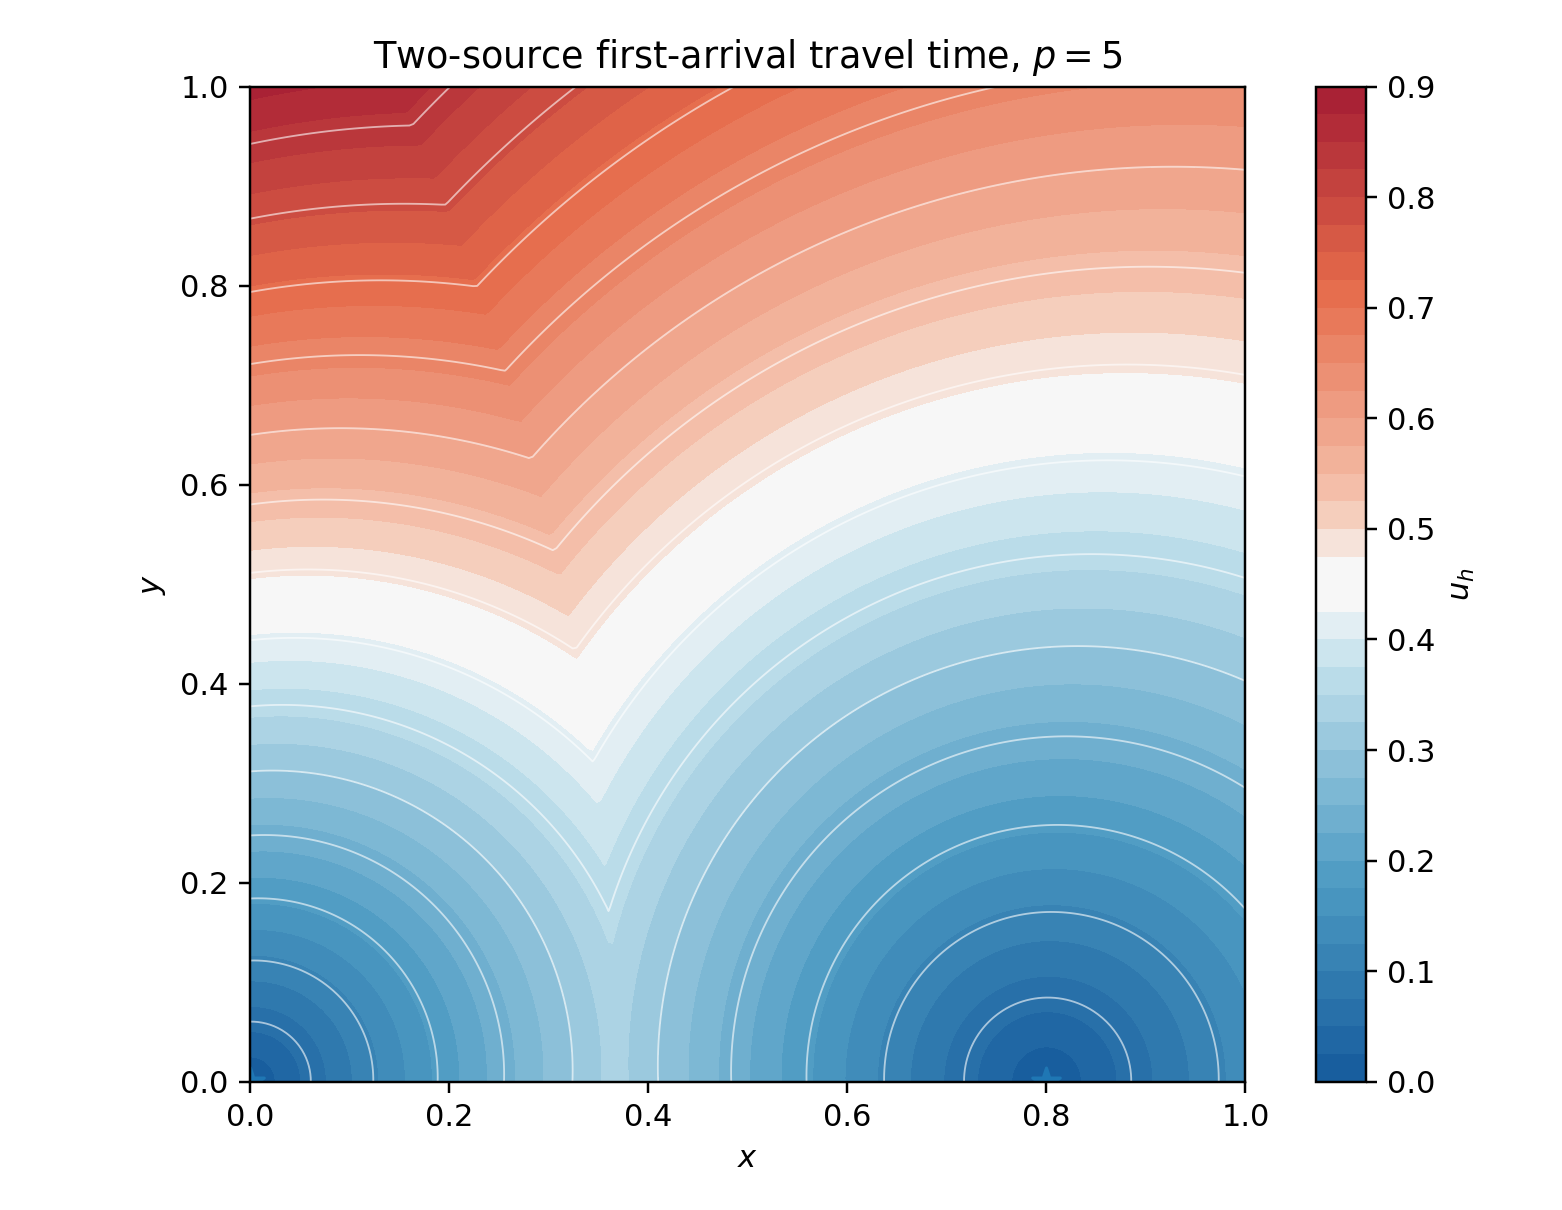
\includegraphics[width=.62\textwidth]{linear_speed_two_source_p5.png}
\caption{Two-source first-arrival phase in the linear-speed medium at $p=5$.  The kink is the branch-switching interface where the two smooth factored travel times are equal; the minimum selects the first-arrival viscosity branch~\cite{CrandallIshiiLions1992}.}
\label{fig:twosource}
\end{figure}

\subsection{Marmousi: causal branch selection followed by Bernstein correction}\label{sec:marmousi}
The Marmousi model is a standard two-dimensional seismic benchmark with strong lateral and vertical velocity variation~\cite{Versteeg1994}.  We use the smoothed $376\times1151$ velocity array on the $9.2\,\mathrm{km}\times3\,\mathrm{km}$ rectangle, with native spacing $8\,\mathrm{m}$ and a surface source at $(4.6,0)\,\mathrm{km}$.  The reference first-arrival field is computed by a first-order four-direction fast sweep on the native grid.  This calculation is used only for error measurement.

The numerical method follows the hybrid interpretation suggested by the preceding experiments.  A deliberately coarse $73\times25$ causal sweep first selects the viscosity branch.  On the native reference grid we define the relative RMS travel-time error as the discrete $\ell^2$ ratio $\norm{u_h-u_{\rm ref}}_{\ell^2}/\norm{u_{\rm ref}}_{\ell^2}$.  The bilinear prolongation of the coarse selector to that grid has relative RMS travel-time error $2.47\times10^{-2}$ and maximum error $5.65\times10^{-2}\,\mathrm{s}$.  We then factor the source singularity additively,
\[
  u(x)=n(x_s)|x-x_s|+\tau_h(x),
\]
and use the coarse causal field only as the initial branch selector.  The Bernstein correction is globally $C^0$, has degree $p=7$, and is continued in $h$ through six meshes.  At each level we perform five inexact Gauss--Newton corrections, with at most 80 LSMR steps in each linearized solve.  The iteration cap is fixed before the refinement sweep: it acts as iterative regularization and prevents the nonmonotone moment problem from drifting to a different classical branch after the causal selector has identified the first arrival.

\begin{table}[t]
\centering
\small
\caption{Smoothed Marmousi first-arrival benchmark at $p=7$.  The six triangulations are traversed by $h$-continuation.  Errors are measured against the native-grid causal reference.}
\label{tab:marmousi}
\begin{tabular}{rrrrrrr}
\toprule
triangles & C$^0$ DOFs & rel. RMS & mean abs. (s) & $L^\infty$ (s) & residual RMS & time (s)\\
\midrule
24  & 645   & $4.28\times10^{-3}$ & $5.18\times10^{-3}$ & $2.33\times10^{-2}$ & $1.41\times10^{-5}$ & 0.04\\
96  & 2465  & $2.68\times10^{-3}$ & $2.67\times10^{-3}$ & $2.30\times10^{-2}$ & $1.42\times10^{-6}$ & 0.12\\
216 & 5461  & $2.49\times10^{-3}$ & $2.12\times10^{-3}$ & $2.30\times10^{-2}$ & $8.13\times10^{-7}$ & 0.28\\
384 & 9633  & $2.45\times10^{-3}$ & $1.87\times10^{-3}$ & $2.30\times10^{-2}$ & $5.13\times10^{-7}$ & 0.71\\
600 & 14981 & $2.46\times10^{-3}$ & $1.86\times10^{-3}$ & $2.30\times10^{-2}$ & $2.99\times10^{-7}$ & 1.19\\
864 & 21505 & $2.50\times10^{-3}$ & $1.93\times10^{-3}$ & $2.30\times10^{-2}$ & $2.29\times10^{-7}$ & 1.61\\
\bottomrule
\end{tabular}
\end{table}

The best global relative RMS error, $2.45\times10^{-3}$, occurs on 384 triangles with 9633 global Bernstein coefficients; the corresponding mean absolute travel-time error is $1.87\,\mathrm{ms}$.  The native reference contains 432776 grid values.  The comparison is not a claim that the Bernstein correction replaces the causal sweep: the coarse sweep supplies branch selection, while the polynomial solve reduces the travel-time error by approximately one order of magnitude at much smaller representation size than the native reference grid.

Figure~\ref{fig:marmousi-combined} shows a second, more important feature.  Beyond 384 triangles the travel-time error stops decreasing even though the Hamiltonian moment residual continues to fall.  This separation is expected for a first-arrival field containing shock curves: the smooth-branch approximation theory does not apply across the viscosity singular set, and reducing a nonmonotone residual there need not reduce the distance to the viscosity solution.  The Marmousi experiment therefore supplies a practical counterpart to the branchwise scope of Theorems~\ref{thm:approx} and~\ref{thm:global}.

\begin{figure}[tbp]
\centering
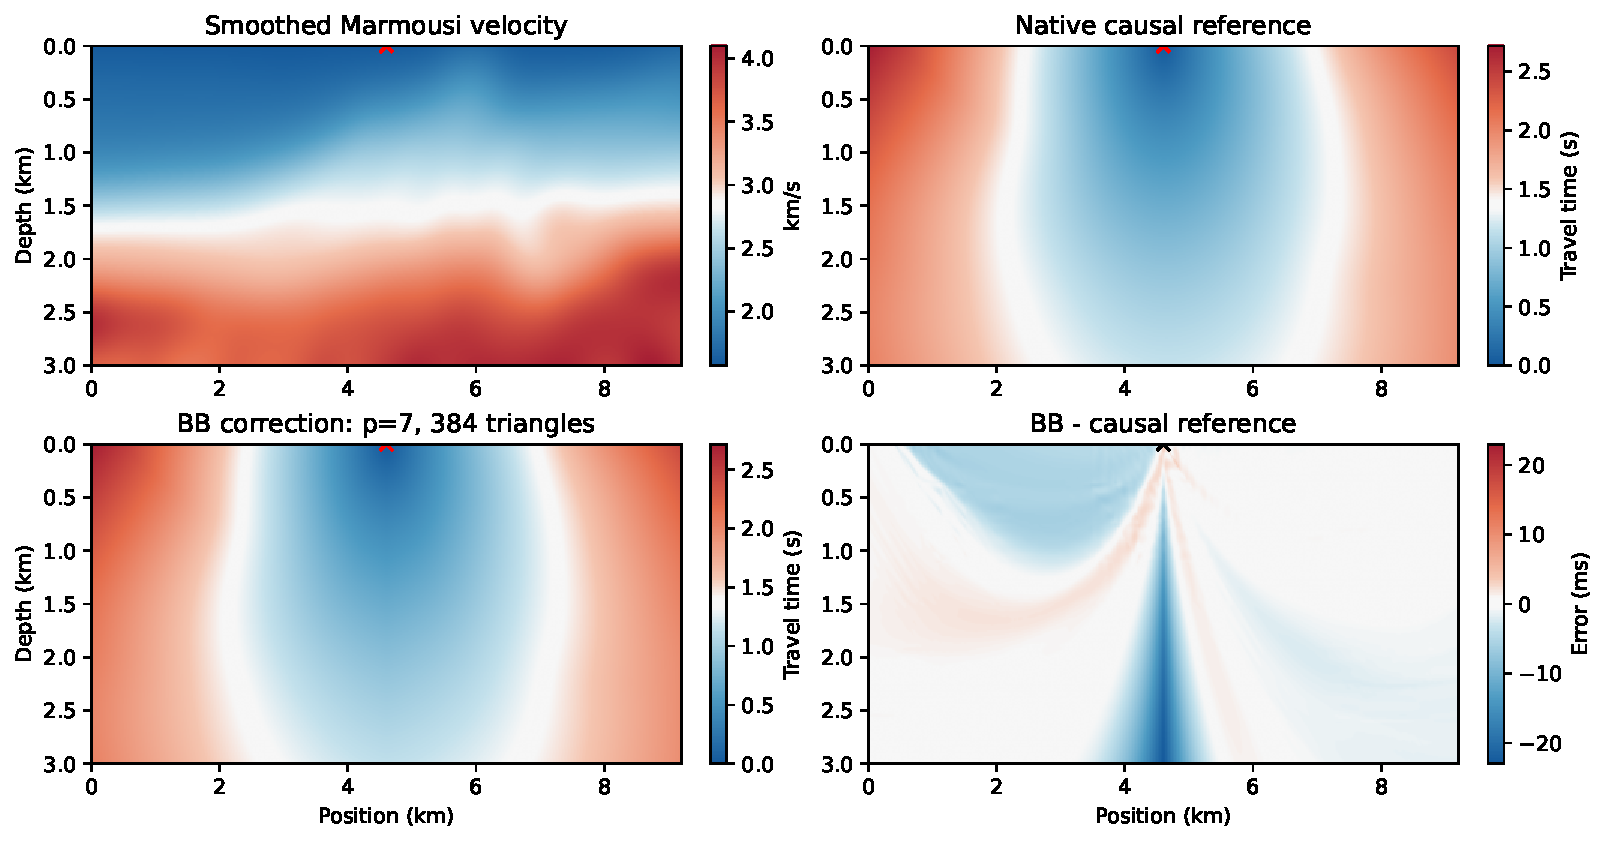
\includegraphics[width=.93\textwidth]{marmousi_smooth_bb_panels.pdf}\\[0.4em]
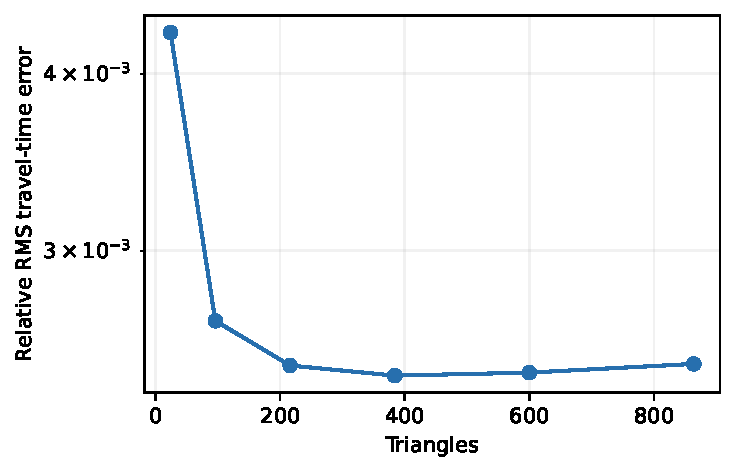
\includegraphics[width=.46\textwidth]{marmousi_h_convergence.pdf}\hfill
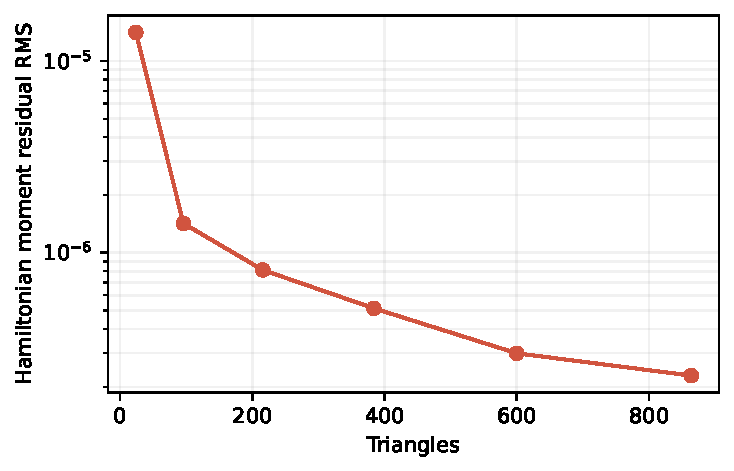
\includegraphics[width=.46\textwidth]{marmousi_residual_convergence.pdf}
\caption{Smoothed Marmousi benchmark and six-level refinement study at $p=7$.  Top block: velocity model, native-grid causal first-arrival reference, $p=7$ Bernstein correction on the $24\times8$ cell mesh (384 triangles), and travel-time error in milliseconds; the marker denotes the surface source.  Bottom left: global relative RMS travel-time error.  Bottom right: Hamiltonian moment residual.  The residual continues to decrease after the travel-time error reaches its first-arrival regularity floor.}
\label{fig:marmousi-combined}
\end{figure}

\subsubsection*{Rough Marmousi at low polynomial order.}
The unsmoothed Marmousi model provides a complementary test in which the velocity contains sharp layer interfaces and the smooth-Hamiltonian assumptions are deliberately violated.  In this regime we do not expect a spectral-in-$p$ branch approximation.  We therefore repeat the same causal initialization and six-level $h$-continuation with the low orders $p=3$ and $p=5$, while retaining $p=7$ only as a comparison of the residual benefit of further enrichment.  Figure~\ref{fig:marmousi-rough} shows the raw model, the causal first-arrival field, and the resulting error curves.

At $p=3$ the relative RMS error decreases from $7.09\times10^{-2}$ on 24 triangles to $5.33\times10^{-2}$ on 864 triangles, using 4033 global coefficients at the finest level.  At $p=5$ the corresponding reduction is from $5.80\times10^{-2}$ to $5.11\times10^{-2}$ with 11041 coefficients.  The $p=7$ sequence reaches $4.44\times10^{-2}$ with 21505 coefficients.  Thus polynomial enrichment still improves the raw-model approximation, but the gain is algebraic and modest compared with the smooth Marmousi case: the coefficient discontinuities, rather than the smooth branch approximation, become the dominant error mechanism.  The $p=3$ and $p=5$ runs therefore provide the relevant low-order baseline for rough media, while $p=7$ quantifies the diminishing return of global enrichment.

\begin{figure}[tbp]
\centering
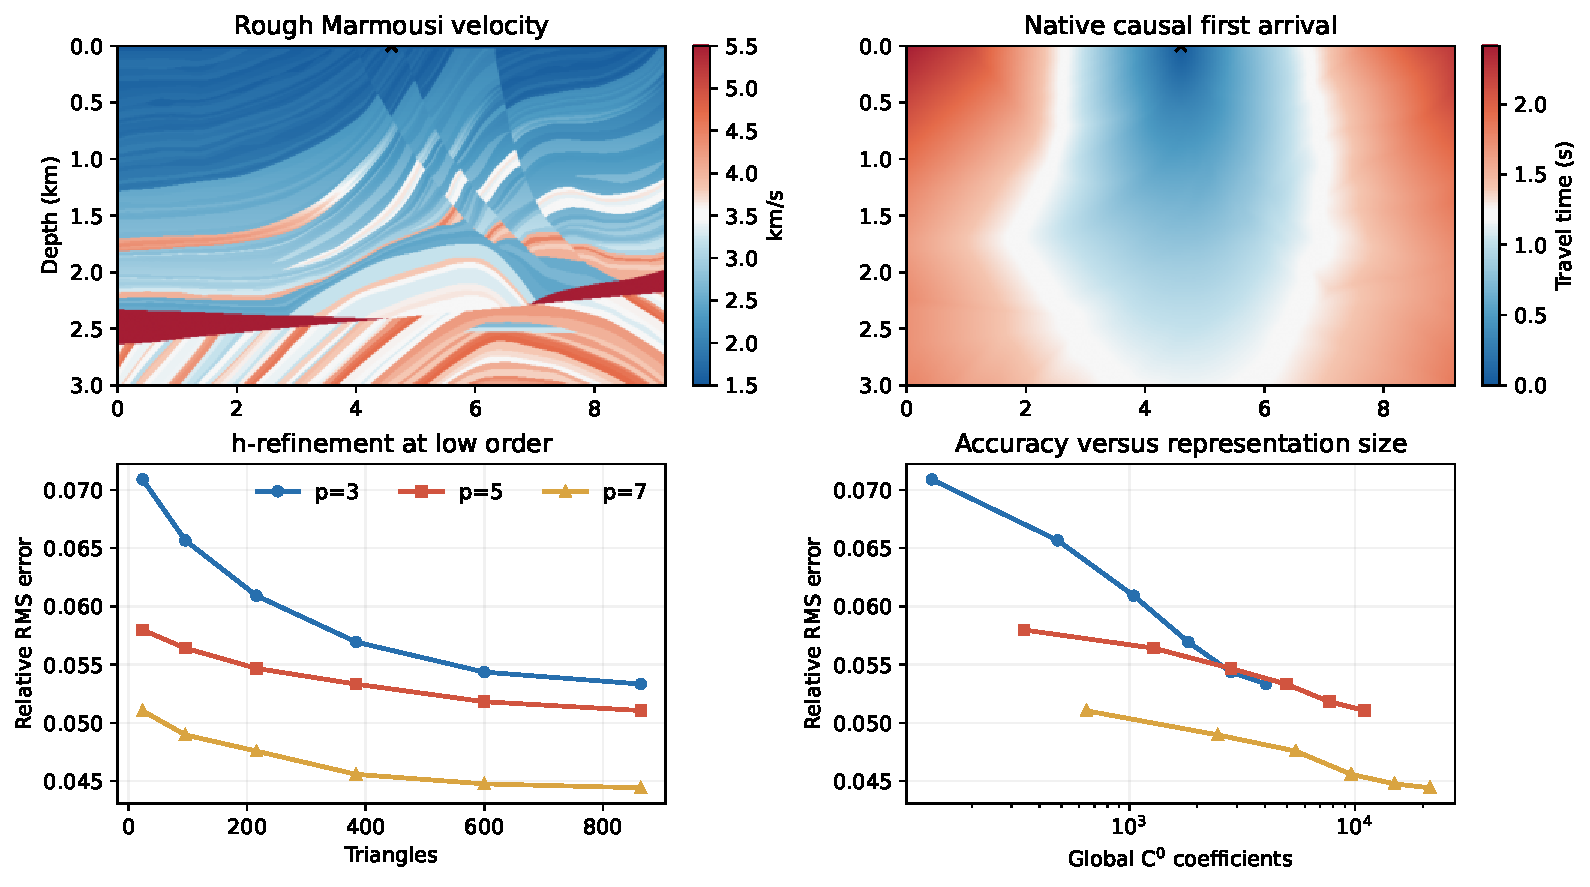
\includegraphics[width=.92\textwidth]{marmousi_raw_lowp.pdf}
\caption{Rough Marmousi with low polynomial order.  Top left: unsmoothed velocity model.  Top right: native-grid causal first-arrival reference.  Bottom left: six-level $h$-refinement for $p=3,5,7$.  Bottom right: the same errors versus global $C^0$ representation size.  The low-order runs remain stable, but the sharp coefficient interfaces prevent the rapid high-order regime observed for the smoothed model.}
\label{fig:marmousi-rough}
\end{figure}

\subsection{Factored focal caustic}\label{sec:focal}
To test focusing explicitly, consider $\Omega=(-1,1)^2$ and
\begin{equation}\label{eq:focalphase}
 u(x,y)=-r+0.035\sin(\pi x)\sin(\pi y),\qquad r=\sqrt{x^2+y^2},
\end{equation}
with $n=\abs{\grad u}$.  The leading phase $-r$ represents inward rays converging to the origin, the elementary local geometry underlying a focal caustic~\cite{EngquistRunborg2003,Runborg2007}.  We factor
\[
 T=-r,\qquad \tau=u-T.
\]
The correction is smooth, while the physical phase retains the focal singularity.  Figure~\ref{fig:focal} shows the computed $p=5$ phase and the six-point odd-degree sweep.  With the embedded qT condensation, the relative $L^2$ error decreases from $1.08\times10^{-4}$ at $p=3$ to $1.15\times10^{-6}$ at $p=5$, $1.40\times10^{-8}$ at $p=7$, and $4.24\times10^{-11}$ at $p=9$, reaching $3.47\times10^{-14}$ at $p=13$.  The relative $H^1$ error at $p=13$ is $5.25\times10^{-12}$.

\begin{figure}[tbp]
\centering
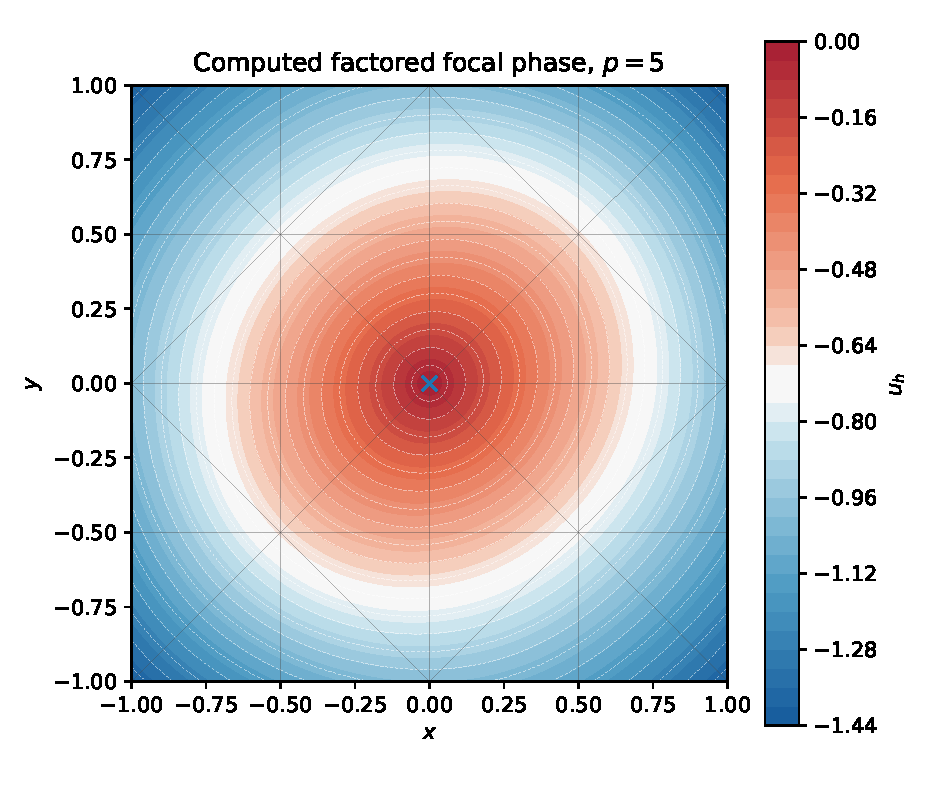
\includegraphics[width=.50\textwidth]{focal_caustic_p5.pdf}\hfill
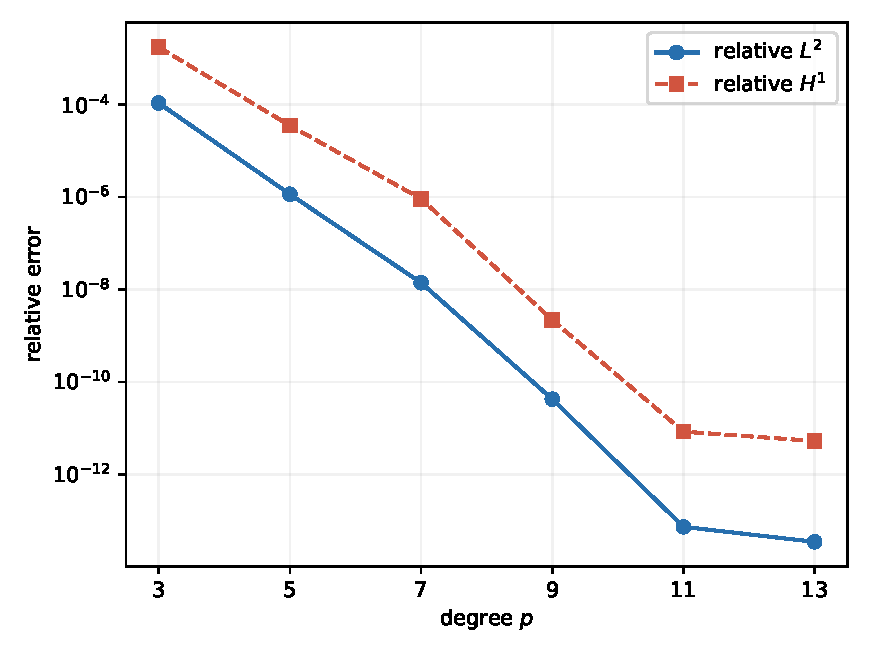
\includegraphics[width=.40\textwidth]{focal_p_convergence.pdf}
\caption{Factored focal test~\eqref{eq:focalphase}. Left: computed phase at $p=5$ on 32 triangles; the marker indicates the focus. Right: the six odd degrees $p=3,5,7,9,11,13$.  The experiment tests a known focal singularity after factoring; it is not a claim of automatic post-caustic branch generation.}
\label{fig:focal}
\end{figure}

\subsection{Very high carrier frequencies}\label{sec:carrier}
In geometrical optics the eikonal equation determines the leading phase independently of the carrier frequency~\cite{EngquistRunborg2003,Runborg2007}.  To measure the high-frequency consequence of phase error, we reconstruct
\[
  U_\omega=e^{\mathrm i\omega u},\qquad
  U_{\omega,h}=e^{\mathrm i\omega u_h}
\]
from the smooth manufactured phase~\eqref{eq:smoothphase}, using the $p=5$, 18-triangle solution whose relative phase $L^2$ error is $6.77\times10^{-7}$.  Table~\ref{tab:omega} and Figure~\ref{fig:omega} contain nine frequencies and extend the reconstruction test to $\omega=20000$.  The relative oscillatory-field error is $1.03\times10^{-2}$ at the largest frequency.

\begin{table}[t]
\centering
\caption{Carrier-frequency amplification of the phase error.}
\label{tab:omega}
\begin{tabular}{rr}
\toprule
$\omega$ & $\norm{e^{\mathrm i\omega u_h}-e^{\mathrm i\omega u}}_0/\norm{e^{\mathrm i\omega u}}_0$\\
\midrule
50    & $2.58\times10^{-5}$\\
100   & $5.17\times10^{-5}$\\
250   & $1.29\times10^{-4}$\\
500   & $2.58\times10^{-4}$\\
1000  & $5.17\times10^{-4}$\\
2000  & $1.03\times10^{-3}$\\
5000  & $2.58\times10^{-3}$\\
10000 & $5.17\times10^{-3}$\\
20000 & $1.03\times10^{-2}$\\
\bottomrule
\end{tabular}
\end{table}

\begin{figure}[tbp]
\centering
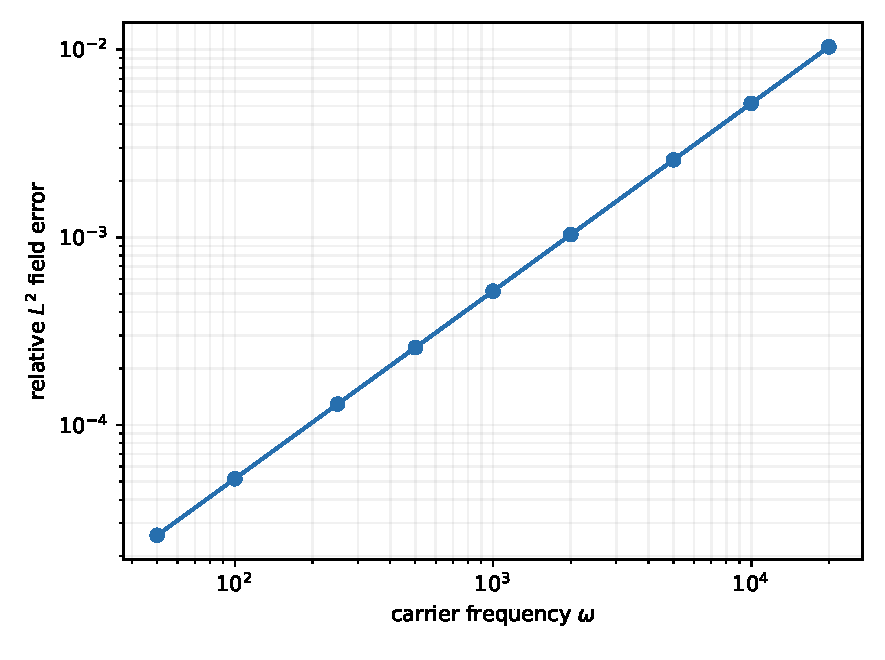
\includegraphics[width=.50\textwidth]{carrier_frequency.pdf}
\caption{Relative error after reconstruction of the oscillatory field $e^{\mathrm i\omega u_h}$.  Nine carrier frequencies are shown; the nearly linear growth is the expected small-phase-error regime.}
\label{fig:omega}
\end{figure}

For small phase error $\delta u=u_h-u$, the identity
\[
 e^{\mathrm i\omega u_h}-e^{\mathrm i\omega u}
 =e^{\mathrm i\omega u}(e^{\mathrm i\omega\delta u}-1)
\]
gives $\abs{e^{\mathrm i\omega\delta u}-1}\le\omega\abs{\delta u}$.  The experiment is therefore a stringent way to report what a seemingly small travel-time error means in a very high-frequency wave calculation.

\FloatBarrier
\section{Discussion}
The two non-eikonal tests confirm the structural point of Sections~\ref{sec:bb}--\ref{sec:approx}: the Bernstein construction depends on the first-order characteristic derivative $H_p$, not on the special quadratic form of the eikonal equation.  Both an anisotropic quadratic Hamiltonian and a quartic convex Hamiltonian show the same degree-convergence pattern as the smooth eikonal branch.  The nonlinear Hamiltonian can therefore be evaluated directly at quadrature points while the sparse $p\to p-1$ Bernstein map is reserved for its derivative data and analytic Jacobian.

The eikonal equation remains the more demanding numerical laboratory because it naturally brings together branch selection, singular point sources, heterogeneous rays, caustics, and high-frequency phase reconstruction.  The smooth and factored examples show that once the active branch is regularized, the high-order polynomial phase can remain accurate enough that $e^{i\omega u_h}$ is useful at carrier frequencies far larger than those at which one would directly approximate the oscillatory wave by global polynomials.  The odd-degree sweeps also show that the sparse continuation implementation remains practical through $p=13$ without forming dense global Jacobians.

The theory also separates three issues that are easily conflated.  Theorem~\ref{thm:approx} is a local approximation result controlled by characteristic transversality and the curvature of the Hamiltonian through $H_{pp}$.  Estimate~\eqref{eq:Hperturb} isolates consistency error from approximating the Hamiltonian itself.  Theorem~\ref{thm:global} concerns the assembled nonlinear branch and exposes the discrete stability factor $\sigma_h$.  None of these statements implies monotone convergence to an arbitrary viscosity solution.  That remains the strength of the established ENO/WENO, causal, DG, and filtered frameworks~\cite{OsherShu1991,SethianVladimirsky2003,Abgrall2009,LepskyHuShu2000,ObermanSalvador2015}.

For the eikonal problem, several limitations are therefore deliberate.  The method does not automatically create multiple phases after a caustic; that requires multivalued geometrical-optics or phase-space machinery~\cite{QianLeung2004,Runborg2007}.  Nonsmooth first arrivals are handled here either by explicit branchwise minima or by known singular factors.  A natural continuation is a hybrid method in which a monotone/causal Hamilton--Jacobi solver identifies branches and singular sets, while the Bernstein moment formulation supplies high-order branchwise correction on smooth regions.

\section{Conclusions}
We have extended the $C^0$ Bernstein quasi-Trefftz construction from the isotropic eikonal equation to stationary Hamilton--Jacobi equations.  Global continuity is imposed first, and the nonlinear Hamiltonian is enforced afterward through degree-$(p-1)$ residual moments.  The $p-1$ level is not an assumed algebraic degree of the nonlinear residual.  It follows from exact Bernstein differentiation and from the first-order linearized characteristic operator $H_p(x,\grad u)\cdot\grad$.  Under characteristic transversality, the deep block is invertible and the regular local moment manifold has tangent dimension $p+1$ in two dimensions.

For twice differentiable Hamiltonians, the approximation analysis shows that the eikonal quadratic remainder is the special case of a general $H_{pp}$ Taylor remainder.  Smooth branches retain the ordinary degree-$p$ $H^1$ and $L^2$ approximation orders after local nonlinear correction.  A separate perturbation estimate accounts for approximate Hamiltonians, and a conditional global bound makes the assembled branch stability depend explicitly on the smallest singular value of the linearized moment map.

The opening rotating-anisotropy experiment directly compares the full $C^0$ parent approximation with the embedded $C^0$-qT manifold.  The defining moment block is solved to roundoff and the remaining global coefficients are reconstructed from retained trace coordinates, while the high-order approximation trend of the parent space is preserved.  The subsequent non-eikonal anisotropic and quartic tests verify the general formulation.  The eikonal equation then serves as the main numerical study, covering exact recovery, smooth high-order convergence, strongly heterogeneous propagation, analytic point sources, a nonsmooth two-source first-arrival interface, a causal-plus-Bernstein Marmousi calculation, a factored focal singularity, and reconstructed waves at carrier frequency 20000.  The most promising use of the method is therefore as a high-order branch solver inside a broader Hamilton--Jacobi workflow.  Future work will combine branch detection with the nonlinear qT condensation, develop $h$--$p$ adaptation driven by the complementary consistency defect and characteristic curvature, and replace the one-time rank-revealing factorization by scalable sparse pivoting on very large meshes.

\section*{Data and code availability}
The source package accompanying this manuscript contains the global $C^0$ Bernstein assembler, the vectorized sparse Hamilton--Jacobi residual/Jacobian driver, degree-elevation and mesh continuation, heterogeneous and factored eikonal benchmark drivers, the Marmousi fast-sweeping reference and Bernstein-correction drivers, the CSV data used in the tables and convergence plots, and the scripts used to generate the numerical figures.  The Marmousi velocity arrays themselves are not redistributed; the benchmark driver accepts externally supplied smooth and original velocity files.

\section*{Funding}
The author received no specific funding for this work.

\section*{Declaration of competing interest}
The author declares no competing interests.

\small
\begin{thebibliography}{99}
\bibitem{CrandallIshiiLions1992}
M.G.~Crandall, H.~Ishii, P.-L.~Lions,
User's guide to viscosity solutions of second order partial differential equations,
\emph{Bull. Amer. Math. Soc.} 27 (1992) 1--67.
\newblock doi:10.1090/S0273-0979-1992-00266-5.

\bibitem{BarlesSouganidis1991}
G.~Barles, P.E.~Souganidis,
Convergence of approximation schemes for fully nonlinear second order equations,
\emph{Asymptotic Analysis} 4 (1991) 271--283.
\newblock doi:10.3233/ASY-1991-4305.

\bibitem{Tsitsiklis1995}
J.N.~Tsitsiklis,
Efficient algorithms for globally optimal trajectories,
\emph{IEEE Trans. Automat. Control} 40 (1995) 1528--1538.
\newblock doi:10.1109/9.412624.

\bibitem{Sethian1996}
J.A.~Sethian,
A fast marching level set method for monotonically advancing fronts,
\emph{Proc. Natl. Acad. Sci. USA} 93 (1996) 1591--1595.
\newblock doi:10.1073/pnas.93.4.1591.

\bibitem{Sethian1999}
J.A.~Sethian,
Fast marching methods,
\emph{SIAM Rev.} 41 (1999) 199--235.
\newblock doi:10.1137/S0036144598347059.

\bibitem{SethianVladimirsky2003}
J.A.~Sethian, A.~Vladimirsky,
Ordered upwind methods for static Hamilton--Jacobi equations: theory and algorithms,
\emph{SIAM J. Numer. Anal.} 41 (2003) 325--363.
\newblock doi:10.1137/S0036142901392742.

\bibitem{Zhao2005}
H.~Zhao,
A fast sweeping method for eikonal equations,
\emph{Math. Comp.} 74 (2005) 603--627.
\newblock doi:10.1090/S0025-5718-04-01678-3.

\bibitem{KaoOsherTsai2005}
C.-Y.~Kao, S.~Osher, Y.-H.~Tsai,
Fast sweeping methods for static Hamilton--Jacobi equations,
\emph{SIAM J. Numer. Anal.} 42 (2005) 2612--2632.
\newblock doi:10.1137/S0036142902419600.

\bibitem{ZhangZhaoQian2006}
Y.-T.~Zhang, H.-K.~Zhao, J.~Qian,
High order fast sweeping methods for static Hamilton--Jacobi equations,
\emph{J. Sci. Comput.} 29 (2006) 25--56.
\newblock doi:10.1007/s10915-005-9014-3.

\bibitem{QianZhangZhao2007}
J.~Qian, Y.-T.~Zhang, H.-K.~Zhao,
Fast sweeping methods for eikonal equations on triangular meshes,
\emph{SIAM J. Numer. Anal.} 45 (2007) 83--107.
\newblock doi:10.1137/050627083.

\bibitem{ChaconVladimirsky2012}
A.~Chacon, A.~Vladimirsky,
Fast two-scale methods for eikonal equations,
\emph{SIAM J. Sci. Comput.} 34 (2012) A547--A578.
\newblock doi:10.1137/10080909X.

\bibitem{OsherShu1991}
S.~Osher, C.-W.~Shu,
High-order essentially nonoscillatory schemes for Hamilton--Jacobi equations,
\emph{SIAM J. Numer. Anal.} 28 (1991) 907--922.
\newblock doi:10.1137/0728049.

\bibitem{BarthSethian1998}
T.J.~Barth, J.A.~Sethian,
Numerical schemes for the Hamilton--Jacobi and level set equations on triangulated domains,
\emph{J. Comput. Phys.} 145 (1998) 1--40.
\newblock doi:10.1006/jcph.1998.6007.

\bibitem{LevyNayakShuZhang2006}
D.~Levy, S.~Nayak, C.-W.~Shu, Y.-T.~Zhang,
Central WENO schemes for Hamilton--Jacobi equations on triangular meshes,
\emph{SIAM J. Sci. Comput.} 28 (2006) 2229--2247.
\newblock doi:10.1137/040612002.

\bibitem{Abgrall1996}
R.~Abgrall,
Numerical discretization of the first-order Hamilton--Jacobi equation on triangular meshes,
\emph{Comm. Pure Appl. Math.} 49 (1996) 1339--1373.
\newblock doi:10.1002/(SICI)1097-0312(199612)49:12<1339::AID-CPA5>3.0.CO;2-B.

\bibitem{HuShu1999}
C.~Hu, C.-W.~Shu,
A discontinuous Galerkin finite element method for Hamilton--Jacobi equations,
\emph{SIAM J. Sci. Comput.} 21 (1999) 666--690.
\newblock doi:10.1137/S1064827598337282.

\bibitem{LepskyHuShu2000}
O.~Lepsky, C.~Hu, C.-W.~Shu,
Analysis of the discontinuous Galerkin method for Hamilton--Jacobi equations,
\emph{Appl. Numer. Math.} 33 (2000) 423--434.
\newblock doi:10.1016/S0168-9274(99)00109-9.

\bibitem{BornemannRasch2006}
F.~Bornemann, C.~Rasch,
Finite-element discretization of static Hamilton--Jacobi equations based on a local variational principle,
\emph{Comput. Vis. Sci.} 9 (2006) 57--69.
\newblock doi:10.1007/s00791-006-0016-y.

\bibitem{ChengShu2007}
Y.~Cheng, C.-W.~Shu,
A discontinuous Galerkin finite element method for directly solving the Hamilton--Jacobi equations,
\emph{J. Comput. Phys.} 223 (2007) 398--415.
\newblock doi:10.1016/j.jcp.2006.09.012.

\bibitem{Abgrall2009}
R.~Abgrall,
Construction of simple, stable, and convergent high order schemes for steady first order Hamilton--Jacobi equations,
\emph{SIAM J. Sci. Comput.} 31 (2009) 2419--2446.
\newblock doi:10.1137/040615997.

\bibitem{ObermanSalvador2015}
A.M.~Oberman, T.~Salvador,
Filtered schemes for Hamilton--Jacobi equations: a simple construction of convergent accurate difference schemes,
\emph{J. Comput. Phys.} 284 (2015) 367--388.
\newblock doi:10.1016/j.jcp.2014.12.039.

\bibitem{FomelLuoZhao2009}
S.~Fomel, S.~Luo, H.~Zhao,
Fast sweeping method for the factored eikonal equation,
\emph{J. Comput. Phys.} 228 (2009) 6440--6455.
\newblock doi:10.1016/j.jcp.2009.05.029.

\bibitem{TreisterHaber2016}
E.~Treister, E.~Haber,
A fast marching algorithm for the factored eikonal equation,
\emph{J. Comput. Phys.} 324 (2016) 210--225.
\newblock doi:10.1016/j.jcp.2016.08.012.

\bibitem{Versteeg1994}
R.~Versteeg,
The Marmousi experience: velocity model determination on a synthetic complex data set,
\emph{The Leading Edge} 13 (1994) 927--936.
\newblock doi:10.1190/1.1437051.

\bibitem{PotterCameron2019}
S.F.~Potter, M.K.~Cameron,
Ordered line integral methods for solving the eikonal equation,
\emph{J. Sci. Comput.} 81 (2019) 2010--2050.
\newblock doi:10.1007/s10915-019-01077-z.

\bibitem{EngquistRunborg2003}
B.~Engquist, O.~Runborg,
Computational high frequency wave propagation,
\emph{Acta Numerica} 12 (2003) 181--266.
\newblock doi:10.1017/S0962492902000119.

\bibitem{Runborg2007}
O.~Runborg,
Mathematical models and numerical methods for high frequency waves,
\emph{Commun. Comput. Phys.} 2 (2007) 827--880.
\newblock doi:10.4208/cicp.2007.v2.p827.

\bibitem{QianLeung2004}
J.~Qian, S.~Leung,
A local level set method for paraxial geometrical optics,
\emph{SIAM J. Sci. Comput.} 28 (2006) 206--223.
\newblock doi:10.1137/030601673.

\bibitem{KapitaC1BernsteinQT2026}
S.~Kapita,
Efficient $C^1$ Bernstein quasi-Trefftz discretization for heterogeneous high-frequency Helmholtz problems,
arXiv:2609.05849 [math.NA], 2026.
\newblock \url{https://arxiv.org/abs/2609.05849}.

\bibitem{Farin2002}
G.~Farin,
\emph{Curves and Surfaces for CAGD: A Practical Guide}, 5th ed.,
Morgan Kaufmann, San Francisco, 2002.

\bibitem{LaiSchumaker2007}
M.-J.~Lai, L.L.~Schumaker,
\emph{Spline Functions on Triangulations},
Cambridge University Press, Cambridge, 2007.

\bibitem{Ciarlet2002}
P.G.~Ciarlet,
\emph{The Finite Element Method for Elliptic Problems},
SIAM, Philadelphia, 2002.
\newblock doi:10.1137/1.9780898719208.

\bibitem{ImbertGerardDespres2014}
L.-M.~Imbert-G\'erard, B.~Despr\'es,
A generalized plane-wave numerical method for smooth nonconstant coefficients,
\emph{IMA J. Numer. Anal.} 34 (2014) 1072--1103.
\newblock doi:10.1093/imanum/drt030.

\bibitem{ImbertGerardMoiolaStocker2023}
L.-M.~Imbert-G\'erard, A.~Moiola, P.~Stocker,
A space-time quasi-Trefftz DG method for the wave equation with piecewise-smooth coefficients,
\emph{Math. Comp.} 92 (2023) 1211--1249.
\newblock doi:10.1090/mcom/3786.

\bibitem{ImbertGerardSylvand2025}
L.-M.~Imbert-G\'erard, G.~Sylvand,
Three types of quasi-Trefftz functions for the 3D convected Helmholtz equation: construction and approximation properties,
\emph{IMA J. Numer. Anal.} 45 (2025) 2274--2328.
\newblock doi:10.1093/imanum/drae060.

\bibitem{ImbertGerardEtAl2025}
L.-M.~Imbert-G\'erard, A.~Moiola, C.~Perinati, P.~Stocker,
Polynomial quasi-Trefftz DG for PDEs with smooth coefficients: elliptic problems,
\emph{IMA J. Numer. Anal.} 45 (2025) 3473--3506.
\newblock doi:10.1093/imanum/drae094.
\end{thebibliography}

\end{document}
